          

\documentclass[journal,onecolumn]{IEEEtran}

\hyphenation{op-tical net-works semi-conduc-tor}
\usepackage[square,sort&compress,numbers]{natbib}
\usepackage[margin=1in]{geometry}
\usepackage{textcomp} 
\usepackage{amssymb}  
\usepackage{bm}       
\usepackage{booktabs}
\usepackage{dcolumn}  
\usepackage{multirow} 
\usepackage{ragged2e}
\usepackage{graphicx} 
\usepackage{float}
\usepackage{rotating}
\usepackage{makecell}
\usepackage{multirow}
\usepackage[english]{babel}
\usepackage{graphicx}
\usepackage{subcaption}
\usepackage{listings}
\usepackage{array}
\usepackage[printonlyused]{acronym}
\usepackage[framed, numbered]{matlab-prettifier}
\usepackage[utf8]{inputenc}
\usepackage[english]{babel}
\usepackage{times}
\usepackage{indentfirst}
\usepackage{multicol}
\usepackage{enumitem}
\usepackage{attachfile}
\usepackage{multirow}
\usepackage{tabularray}

% Table Stuff
\newcommand{\spheading}[2][9.5em]{% \spheading[<width>]{<stuff>}
	\rotatebox{90}{\parbox{#1}{\raggedright #2}}}

\begin{document}
	%
	% paper title
	% Titles are generally capitalized except for words such as a, an, and, as,
	% at, but, by, for, in, nor, of, on, or, the, to and up, which are usually
	% not capitalized unless they are the first or last word of the title.
	% Linebreaks \\ can be used within to get better formatting as desired.
	% Do not put math or special symbols in the title.
	\title{Enhance Road Detection Data Processing of LiDAR Point Clouds to Specifically Identify Unmarked Gravel Rural Roads}
	%
	%
	% author names and IEEE memberships
	% note positions of commas and nonbreaking spaces ( ~ ) LaTeX will not break
	% a structure at a ~ so this keeps an author's name from being broken across
	% two lines.
	% use \thanks{} to gain access to the first footnote area
	% a separate \thanks must be used for each paragraph as LaTeX2e's \thanks
	% was not built to handle multiple paragraphs
	%
	
	\author{Rhett Huston, Jay Wilhelm}
%	{
%		and~Jane~Doe,~\IEEEmembership{Life~Fellow,~IEEE}% <-this % stops a space
%		\thanks{M. Shell was with the Department
%			of Electrical and Computer Engineering, Georgia Institute of Technology, Atlanta,
%			GA, 30332 USA e-mail: (see http://www.michaelshell.org/contact.html).}% <-this % stops a space
%		\thanks{J. Doe and J. Doe are with Anonymous University.}% <-this % stops a space
%		\thanks{Manuscript received April 19, 2005; revised August 26, 2015.}}
	
	% note the % following the last \IEEEmembership and also \thanks - 
	% these prevent an unwanted space from occurring between the last author name
	% and the end of the author line. i.e., if you had this:
	% 
	% \author{....lastname \thanks{...} \thanks{...} }
	%                     ^------------^------------^----Do not want these spaces!
	%
	% a space would be appended to the last name and could cause every name on that
	% line to be shifted left slightly. This is one of those "LaTeX things". For
	% instance, "\textbf{A} \textbf{B}" will typeset as "A B" not "AB". To get
	% "AB" then you have to do: "\textbf{A}\textbf{B}"
	% \thanks is no different in this regard, so shield the last } of each \thanks
% that ends a line with a % and do not let a space in before the next \thanks.
% Spaces after \IEEEmembership other than the last one are OK (and needed) as
% you are supposed to have spaces between the names. For what it is worth,
% this is a minor point as most people would not even notice if the said evil
% space somehow managed to creep in.



% The paper headers
\markboth{Some Sort of Journal}%
{Shell \MakeLowercase{\textit{et al.}}: Bare Demo of IEEEtran.cls for IEEE Journals}
% The only time the second header will appear is for the odd numbered pages
% after the title page when using the twoside option.
% 
% *** Note that you probably will NOT want to include the author's ***
% *** name in the headers of peer review papers.                   ***
% You can use \ifCLASSOPTIONpeerreview for conditional compilation here if
% you desire.




% If you want to put a publisher's ID mark on the page you can do it like
% this:
%\IEEEpubid{0000--0000/00\$00.00~\copyright~2015 IEEE}
% Remember, if you use this you must call \IEEEpubidadjcol in the second
% column for its text to clear the IEEEpubid mark.



% use for special paper notices
%\IEEEspecialpapernotice{(Invited Paper)}




% make the title area
\maketitle

% As a general rule, do not put math, special symbols or citations
% in the abstract or keywords.
\begin{abstract}
	
	{Gravel and chipseal roads that lack standardized features such as curbs or painted lines present detection and navigation challenges to autonomous vehicles. Differentiation between road surfaces and surrounding terrain is necessary to determine boundaries for trajectory tracking and navigation. Global Positioning Service (GPS) and high resolution maps cannot be relied upon for navigation of rural roads, as some may only be width of the vehicle and GPS may not be accurate enough. Normal Distribution Transform (NDT) based on scanning LiDAR data may be insufficient for navigating on gravel roads. This work will examine a method of classifying scanning LiDAR data spatial and remission features for explicit detection of unmarked gravel and chipseal road surfaces. Exploration of terrain classification using high resolution scanning LiDAR data of these road surfaces will allow for predicting road boundary location potentially enabling confident autonomous operations on gravel roads. The principal outcome of this work is a method for gravel road detection using LiDAR data for the purpose of predicting road boundary locations. Detection of unmarked road surfaces would increase the operational region capabilities of self driving vehicles considerably by allowing autonomous operations on 1.5 million miles of previously undetected roads.}
	
\end{abstract}

%	
%	% Note that keywords are not normally used for peerreview papers.
%	\begin{IEEEkeywords}
%		IEEE, IEEEtran, journal, \LaTeX, paper, template.
%	\end{IEEEkeywords}
%	
%	
%	
%	

\section{Introduction}
	
	% Autonomous vehicles have difficulty detecting rural unpaved gravel roads due to lack of standardized features such as curbs and painted lane lines. 
	%	Autonomous vehicles have relied upon standardized road features such as curbs and painted lane lines or high definition maps paired with precision GPS for navigational solutions. 
	
	% Current methods of road surface analysis rely on cameras and Light Detection and Ranging (LiDAR) sensors to detect standardized road features, however on gravel roads such attributes are non-existent \cite{skorseth_gravel_nodate}.
	
	{LiDAR has been used by autonomous vehicles for road edge detection purposes, however challenges arise in environments with unpaved gravel and chipseal roads due to the lack of standardized road features such as curbs and painted lane lines. Gravel roads comprise 34.8\% \cite{road_stats_2} of all road surfaces in the United States. Some nations have predominately unpaved road networks, such as India, where 70.7\% of all roads by mile are categorized as unpaved \cite{malik_lal_2019}. Detection of unmarked roads may allow for expansion of current civilian autonomous vehicle capabilities as well as introduce opportunities for industries that operate in rural areas. Global Positioning Service (GPS) and high resolution maps cannot be relied upon for navigation of rural roads, as some gravel roads may only be width of the vehicle and GPS is not accurate enough or may not have a reliable signal for precision driving \cite{noauthor_gpsgov_nodate}. Systems that rely on cameras may fail when analyzing gravel roads, as these lack visual cues such as painted lane markings \cite{crisman_scarf_1993} and may in some circumstances closely resemble surrounding terrain. LiDAR point cloud processing systems depend upon distinct geometric features, most commonly curbs \cite{yadav_extraction_2017,liu_new_2013,qiu_fast_2016,fernandes_road_2014,seker_experiments_nodate,yang_semi-automated_2013,miyazaki_line-based_2014,hervieu_road_2013,smadja_road_nodate}, however as curbs are not installed on rural gravel roads \cite{skorseth_gravel_nodate} this method breaks down. Normal Distribution Transform (NDT) scan matching analytically compares two point cloud data sets to track current position, however this model relies on distinct geometric features, and suffers when distinguishing between terrain types making it insufficient for determining road boundaries \cite{biber_normal_2003}. Using 2D projection of planes unto a 3D point cloud of a road surface is an alternative approach, but likewise requires curbs or painted lines for road boundary definition \cite{fernandes_road_2014, borkar_robust_2009-1, guo_lane_2015}. Instead, using a LiDAR forward approach may overcome difficulties in achieving real-time detection of unmarked roads by using terrain classification to discover road type, boundaries, and intersections.} 
	
	

	%Real time description of surface noise based on incoming LiDAR data, then subsequent comparison to a standard, is a possible alternative that may allow for computationally efficient road surface detection. Overlaying camera imagery data with LiDAR allows for assigning incoming LiDAR data with color information, potentially increasing efficiency by narrowing the search area.
	
	{Detection of unmarked road surfaces may rely on the roughness properties without relying on distinct markings or topographical features. Surface roughness is a measurable property that may be used to characterize a gravel road, as they are typically consistent with gravel type used \cite{skorseth_gravel_nodate} which may be exploited in a search and compare function, and is distinct from grass and other ground types \cite{wan_road_2007, levi_3d_2012_light, levi_3d_2012_terrain}. Surface roughness properties may be derived from processing LiDAR spatial and remission data from an aerial and surface level perspective \cite{wan_road_2007, levi_3d_2012_light, levi_3d_2012_terrain, pollyea_experimental_2012,rychkov_computational_2012,lague_accurate_2013,brubaker_use_2013,turner_estimation_2014,campbell_lidar-based_2017,shepard_roughness_2001,tegowski_statistical_2016,sock_probabilistic_2016,milenkovic_roughness_2018,yadav_extraction_2017, yadav_rural_2018}. Implementing a terrain classification model using Random Decision Forests (RDF) using scanning LiDAR data to exploit surface roughness was studied for road surface detection in this study.}
		
	{Evaluation of the detection model will rely principally upon accuracy and processing time, as a moving vehicle must obtain reliable information of the road surface in a timely manner in order to inform trajectory updates, or else risk suffering an accident. Problem Statement: Determine a processing method for increasing road detection precision of unmarked gravel rural roads.}
		
\subsection{Related Work}
	
	{Current LiDAR based road surface detection models may be categorized into two methodologies. Firstly is the analysis of road surface properties, which considers aspects such as topology and surface roughness. Detection based on road surface smoothness was studied by segmenting the point cloud into candidate road surface regions and searching for elevation jumps \cite{liu_new_2013}. Secondly is the detection of roadside curbs, which relies upon the height difference between the road surface and the curb for road edge detection. LiDAR point density at a curb's upper and lower edges can be used to indicate road edges \cite{ibrahim_curb-based_2012}. Fernandes et al. propose a road surface detection method using LiDAR \cite{fernandes_road_2014}, by projecting a 2D reference plane unto the 3D LiDAR data. In this study, road surfaces are assumed to be flat regions between two elevated regions such as curbs. Cameras have been used to supplement LiDAR point cloud data, which can implement 3D colored elevation maps to match pre-stored geometry data in a modified Iterative Closest Point (ICP) algorithm \cite{manz_detection_2011}. Supervised Classification Applied to Road Following (SCARF) is an algorithm that detects road surfaces based on color differences between the road and the surrounding terrain \cite{crisman_scarf_1993}. It was found that difficulties arise when detecting road surfaces in less colored environments \cite{crisman_scarf_1993,manz_detection_2011}.}
	
	{Real time processing of rural gravel roads cannot rely on normalized, consistent features found on urban roads such as curbs, as rural roads lack these features \cite{skorseth_gravel_nodate}. As such, many of the proposed models are rendered unserviceable, as they rely on curbs or painted lines to offer distinctions in data sets \cite{yadav_extraction_2017,liu_new_2013,qiu_fast_2016,fernandes_road_2014,seker_experiments_nodate,yang_semi-automated_2013,miyazaki_line-based_2014,hervieu_road_2013,smadja_road_nodate}.}
	
	{Further limitations are imposed when considering data set size and processing speed. Real time analysis of road surfaces dictates that trajectory updates to the vehicle in motion must have a rapid update rate, which prohibits the relatively lengthy collection of large data sets or any form of post-processing. Proposed methods \cite{yadav_extraction_2017,yadav_road_2018,yadav_rural_2018,yadav_pole-shaped_2015,miyazaki_line-based_2014,yang_semi-automated_2013,liu_new_2013,qiu_fast_2016} do not indicate the minimum number of points required for road surface detection, however large data sets numbering many millions of points are used in those studies. Computation efficiency of road surface detection is mentioned only by a few studies, such as the one completed by Yadav et al \cite{yadav_road_2018}. Principal component analysis on the height of each LiDAR data point was proposed to detect a straight, curb-less rural road with low computation time \cite{yadav_road_2018}. However a computational time of 24 minutes was required to process a 156 meter stretch of road, rendering real time detection impossible.}
	
	% Current literature proposes multiple methods of terrain classification using LiDAR and RGB cameras, and may be roughly broken into two areas of application. Traversability or trafficability is the analysis of generally unstructured environments that includes obstacles or rough terrain types for autonomous vehicle path finding solutions  \cite{schilling_geometric_2017,ojeda_terrain_2006,coombs_driving_2000,stavens_self-supervised_nodate,belter_rough_2010,bartoszyk_terrain-aware_2017,noauthor_fusion_nodate,li_rugged_2019,wilson_terrain_2014,siva_robot_2019}. While this research may be useful for detection of obstacles on the road for the proposed work, it is assumed that the roads that will be studied will be free of obstacles.
	
	{Classification of the surrounding environment is an integral part to the proposed work, as differentiation of gravel road surfaces and surrounding terrain is necessary to determine road boundaries. Terrain classification is the analysis of the ground surface in order to specify the ground surface type \cite{laible_3d_2012,laible_terrain_2013,laible_map_building,rasmussen_combining_2002,reymann_improving_2015,walas_terrain_2014,wietrzykowski_boosting_2014,wang_road_nodate}. LiDAR and camera based real-time terrain classification was studied by projecting a 2D plane unto the point cloud data using a variant of Random Sample Consensus (RANSAC) called M-estimator Sample Consensus (MSAC) \cite{mijakovska_generating_2014} that is built for a more robust result \cite{laible_3d_2012,laible_map_building,laible_terrain_2013}. After segmenting the plane into cells, roughness and intensity histograms were analyzed on a per-cell basis. Markov Random Field (MRF) \cite{chellappa_classification_1985} and Conditional Random Field (CRF) \cite{wallach_conditional_nodate} were compared in their ability to compare individual cells with neighboring cells. Comparison with neighboring cells increases classification type accuracy, as adjacent cell are likely to have the same terrain type \cite{haselich_terrain_2011,zhao_fusion_2014}. It was found that CRF was better suited for classification.	Random Forest (RF) classification showed good results for identification of analysis of LiDAR and camera data \cite{breiman_random_2001}, and was used to predict cell terrain into one of five types, including gravel and grass. It was found that characterizing the LiDAR intensity as Gaussian distributed noise yielded poor results with only a 49.5\% true positive rate, however a low-resolution LiDAR was used. Higher resolution LiDAR that produces a high density point cloud, such as the Velodyne VLP-32 that will be used in the proposed work \cite{vlp_32c}, may allow for better terrain classification with Gaussian characterization of return intensity and spatial data. While capable of real-time classification of terrain type, this method was not employed in road identification and used a low resolution LiDAR system.}
	
	{Neural networks and similar machine learning tools may be used in terrain and road identification. Road classification with LiDAR spacial and remission features was completed with Neural Network classifier, Naive Bayes classifier, and Support Vector Machines (SVM) \cite{wang_road_nodate,wang_two-stage_2018}. Gravel roads were successfully identified with a 98.5\% true positive identification rate, however data collected required post processing. MATLAB's Neural Network tools were used in autonomous road identification using LiDAR and Camera data \cite{rasmussen_combining_2002}, however post processing was required, with unknown computational time.  Terrain classification was completed using Support Vector Machine (SVM), a classification algorithm where a line is drawn between two different categories to differentiate between them \cite{breiman_random_2001}. Histograms and averages for image hue, saturation, and color value, along with LiDAR intensity were used as points of classification for different terrain types. Although a 96\% true positive rate was reported for a rocky surface, the overall process was computationally expensive with 1.8 seconds per image.}
	
	{MLS and RANSAC were compared as methods to project a two dimensional plane unto a point cloud, facilitating examination of points by providing a frame of reference \cite{miller_method_nodate, gojcic_perfect_2019}. Method of least-squares analyses uses regression to approximate the best fit to a data set (\ref{eqn:MLS}). RANSAC is an iterative algorithm that is designed to handle large numbers of outliers in the sample data set \cite{derpanis_overview_nodate,yaniv_random_2010,fischler_random_1987,cantzler_random_nodate}. 
	RDFs are a supervised machine learning method that operates on a set of decision trees \cite{ho_random_1995}. REFs have been shown to be useful with handling LiDAR data sets \cite{breiman_random_2001}, and have been employed in terrain classification \cite{laible_3d_2012,laible_map_building,laible_terrain_2013,khan_high_2011,reymann_improving_2015,schilling_geometric_2017, wietrzykowski_context-aware_2019}. Multiple decision trees are created with bootstrapped data sets - randomly selected data sub-sets from a training set. Classification was determined by the majority results as opposed to the mean \cite{breiman_random_2001,ho_random_1995}. RDFs may be used to predict road surface area by detecting gravel terrain.}

\section{Methodology}

	{Required physical data was gathered by the Hexegon Chrysler Pacifica New Eagle DBW van (Figure \ref{fig:van}), built by AutonomouStuff, owned and operated by Ohio University. LiDAR point cloud data was gathered with the vehicle's roof-mounted Velodyne VLP-32C (Figure \ref{fig:vlp32mount}). Velodnyne's VLP-32C has 32 channels producing 300,000 points per second with a vertical field of view from -45$^{\circ}$ to $+$15$^{\circ}$, providing a high output data stream \cite{vlp_32c}. GPS data was recorded with a PwrPak 7D-E2, a Global Navigation Satellite System (GNSS) \& Inertial Navigation System (INS) manufactured by Novatel, and two GNSS-502 antennas by NavtechGPS. Data acquisition and recording was completed on the vehicle's integrated Ubuntu 18.04 system using Robotic Operating System (ROS). Scanning LiDAR training data was collected on various roads and lots near Athens, Ohio. Scanning LiDAR data of gravel surfaces was gathered principally from an un-named gravel road near Armig Road (Figure \ref{fig:Armig_Road_Camera_View})and a gravel lot maintained by the Ohio University Civil Engineering Department near Blackburn Road. Additional gravel road data for testing purposes only was gathered on Sturbois Road. Scanning LiDAR data of chipseal surfaces was gathered principally from Bean Hollow Road. Additional chipseal road data for testing purposes only was gathered on later portions of both Bean Hollow Road (Figure \ref{fig:Bean_Cam_View}). Scanning LiDAR data of grassy surfaces and foliage was gathered from the sides of the previously stated roads, therefore no special data collection drive was made for those terrain types.}
	
	\begin{figure}[H] 
		\centering
		\begin{subfigure}{0.45\textwidth}
			\centering
			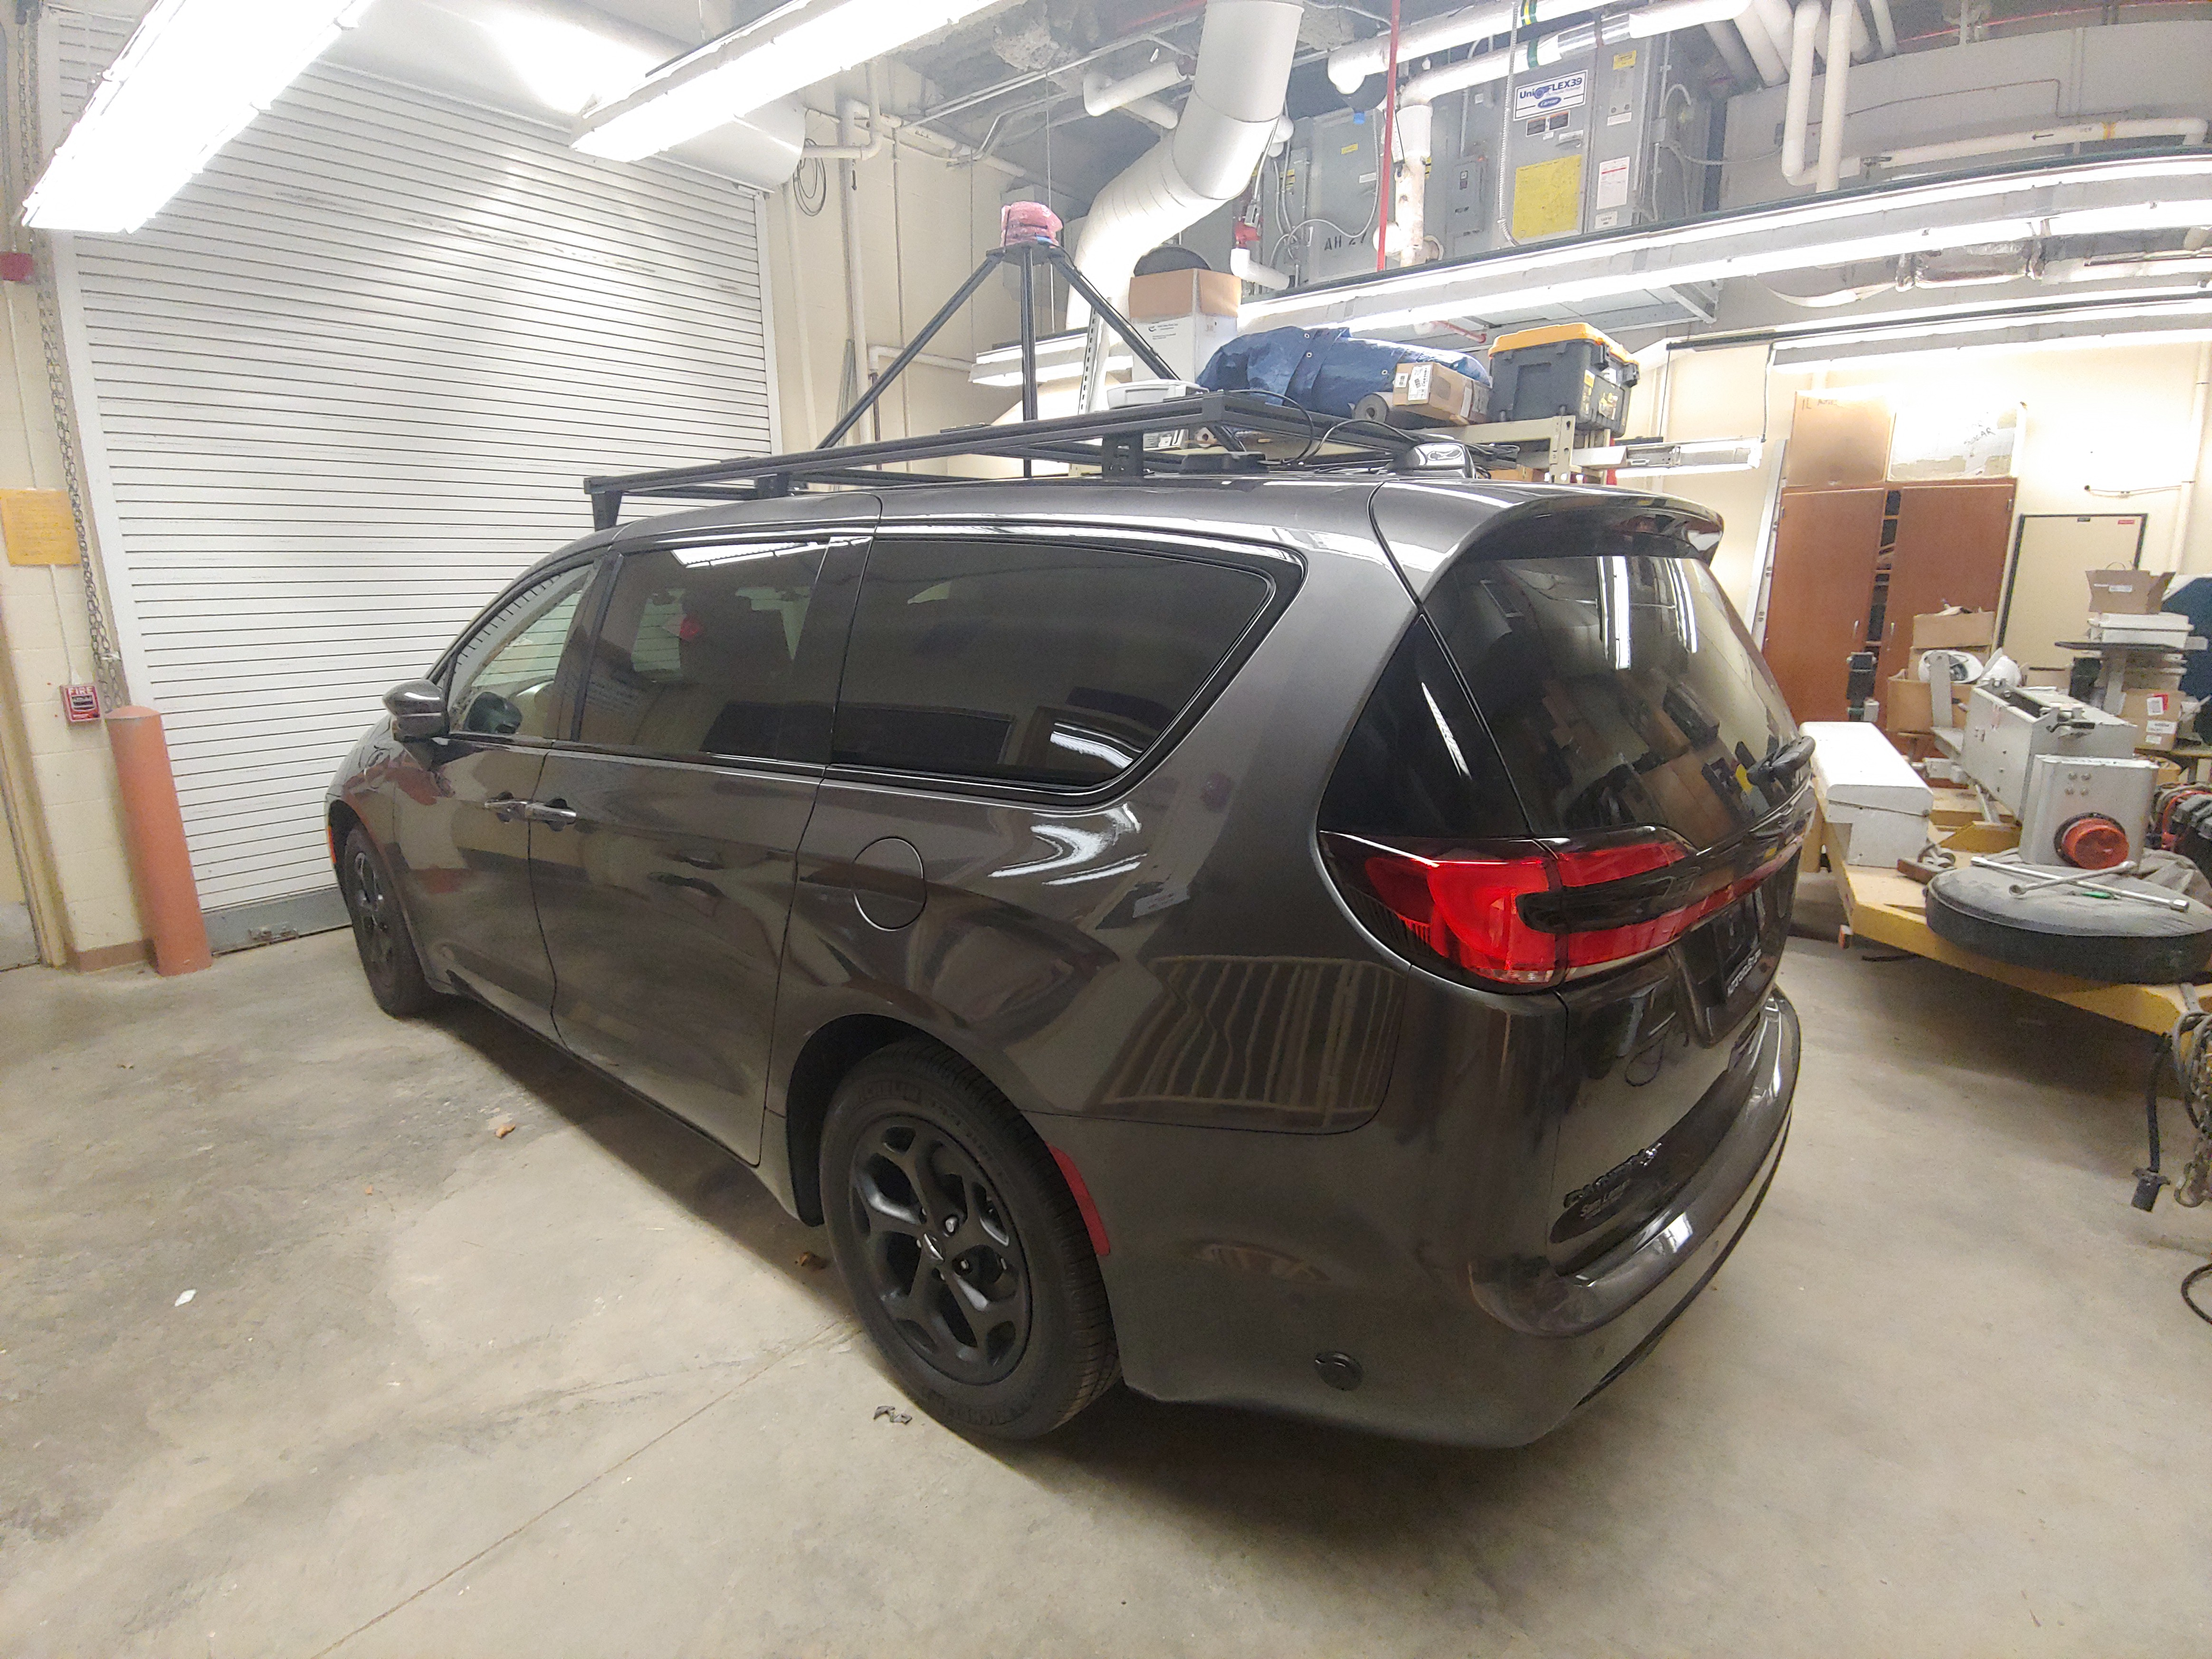
\includegraphics[width=0.9\linewidth,height=4.60 cm,keepaspectratio]{figures/Van}
			\caption[Sensor Van]{}
			\label{fig:van}
		\end{subfigure}
		\begin{subfigure}{0.45\textwidth}
			\centering
			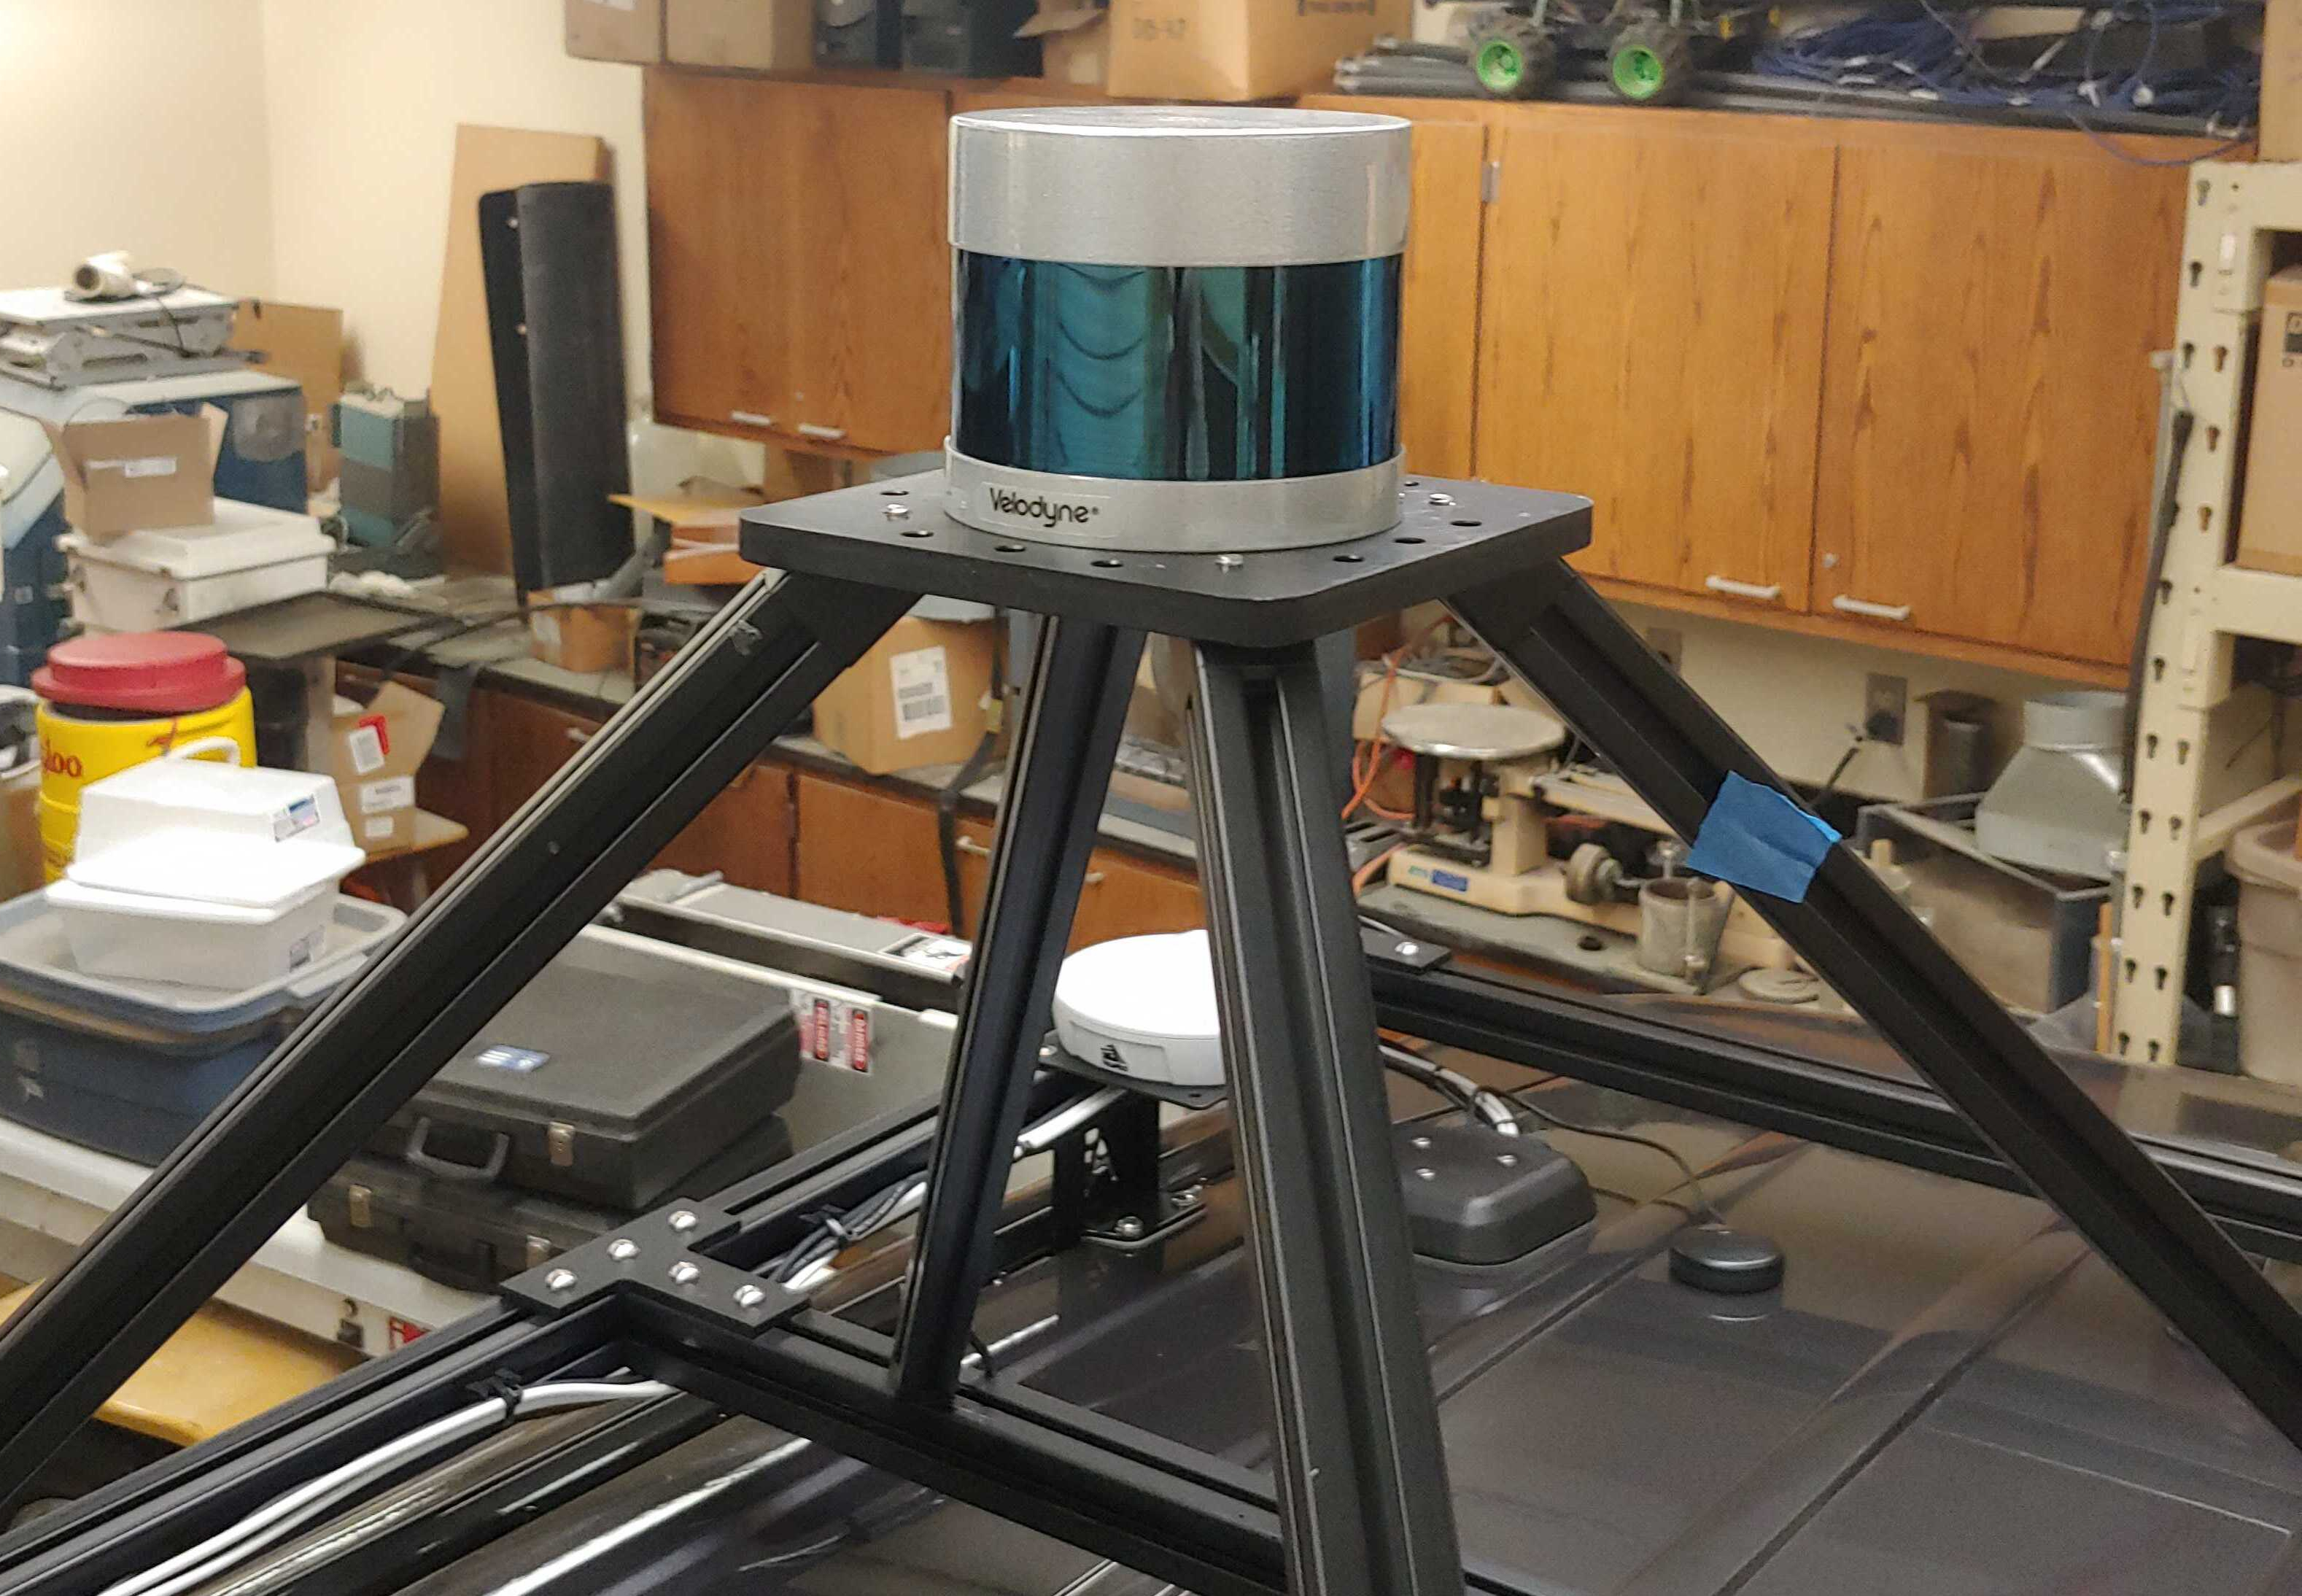
\includegraphics[width=0.9\linewidth,height=4.60 cm,keepaspectratio]{figures/vlp_32_mount_2}
			\caption[VLP 32 on Van]{}
			\label{fig:vlp32mount}
		\end{subfigure}
		\caption[Experimental Apparatus]{Experimental Apparatus (a). Velodyne VLP-32 Scanning LiDAR is mounted on top of the vehicle (b).}
		\label{fig:Experimental_Apperatus}
	\end{figure}

	\begin{figure}[H]
		\centering
		\begin{subfigure}{0.45\textwidth}
			\centering
			\includegraphics[width=1.0\linewidth,height=5.0 cm,keepaspectratio]{figures/Bean_Hollow_Road_Camera}
			\caption[Bean Hollow Road Camera View]{}
			\label{fig:Bean_Cam_View}
		\end{subfigure}
		\begin{subfigure}{0.45\textwidth}
			\centering
			\includegraphics[width=1.0\linewidth,height=5.0 cm,keepaspectratio]{figures/armig_2}
			\caption[Armig Road Camera View]{}
			\label{fig:Armig_Road_Camera_View}
		\end{subfigure}
		\caption[Armig Road \& Bean Hollow Road]{Typical examples of unmarked gravel and chipseal roads. Road view of Bean Hollow Road - an unmarked chipseal road (a). Road view of Armig Road - an unmarked gravel road (b).}
		\label{fig:Combined_Roads}
	\end{figure}

	{MATLAB was used to process the gathered rosbag files using the MATLAB ROSBAG library. Rosbags were directly loaded into the MATLAB environment. Point cloud topic was defined, and the point cloud messages were read from the topic and imported as a data structure. Cartesian coordinates and corresponding intensity values were extracted and saved to disk. GPS and IMU data was extracted in a similar manner. GPS and IMU topics were defined, and topic messages are read. Longitude, latitude, and altitude were extracted from the GPS messages, while roll, pitch, and yaw were extracted from the IMU messages.}
	
	{Scanning LiDAR training and verification data was extracted by selecting appropriate consecutive points from a single LiDAR channel lying on gravel, chipseal, foliage, and grass surfaces. Number of points included in each training data set was not controlled. Foliage was defined as trees and bushes, while grass was defined as a trimmed lawn. Projection of a plane was necessary to provide a reference point for describing point variance. RANSAC and Method of Least Squares were tested for use as plane projection methods. Additionally, a point's perpendicular distance as well as range from the LiDAR origin (Figure \ref{fig:xy_vs_range}) was also considered, both of which has a computational advantage over the plane projection method in that they may be read directly from the Velodyne VLP-32 data stream.}
	
	{RANSAC was implementing by a built-in MATLAB function, $pcfitplane$. Method of Least Squares was implemented by importing a MATLAB library \cite{noauthor_object-oriented_nodate}. Point clouds are individually imported into the MATLAB environment. RANSAC or Method of Least Squares may be used to project a reference plane unto the point cloud. Displaying the point cloud is completed using MATLAB's $pcshow$ function. Training data is selected by manually drawing an area around appropriate points of a desired terrain type using MATLAB's $drawrectangle$ function (Figure \ref{fig:Rectangle_ROI}). Indices for the rectangle are extracted, and MATLAB's function $findPointsInROI$ is used to extract sympatric points within the drawn rectangle (Figure \ref{fig:ROI_Points}). Captured points are then saved to disk along with the projected plane's normal vector and distance from the origin $[a,b,c,d]$.}
	
	\begin{figure}[H]
		\centering
		\begin{subfigure}{0.45\textwidth}
			\centering
			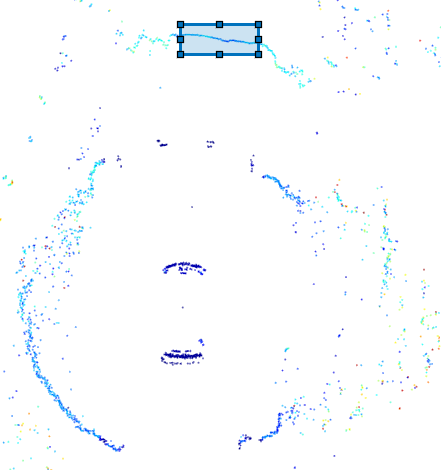
\includegraphics[width=0.5\linewidth]{figures/Rectangle_ROI}
			\caption[Region of Interest Selection]{MATLAB was used to select training data using the $drawrectangle$ function and extracting points that lay within the defined area.}
			\label{fig:Rectangle_ROI}
		\end{subfigure}
		\begin{subfigure}{0.45\textwidth}
			\centering
			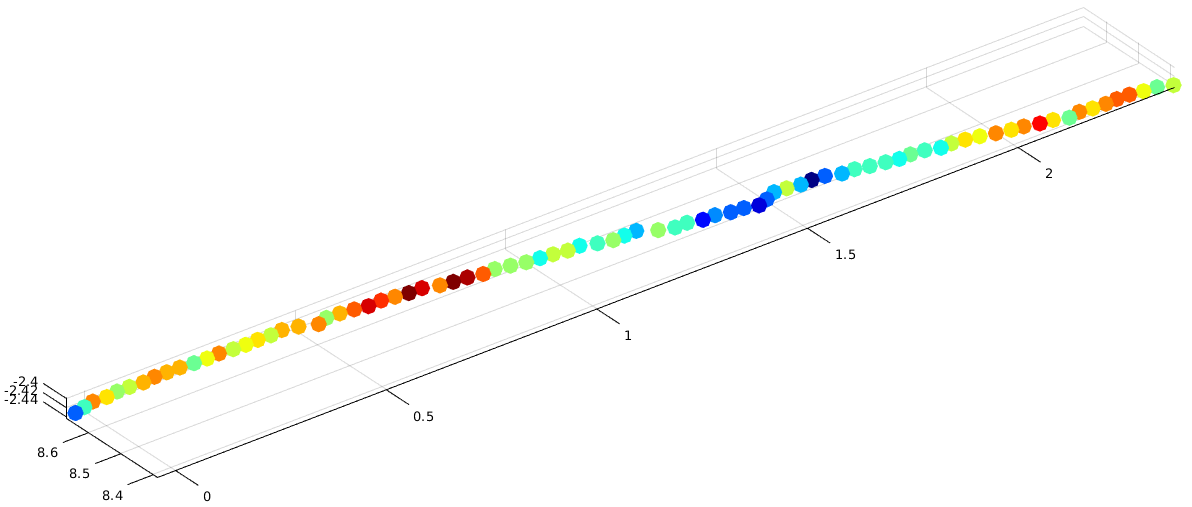
\includegraphics[width=0.5\linewidth]{figures/ROI_Points}
			\caption[Points in Region of Interest]{Selected points (Figure \ref{fig:Rectangle_ROI}) lying on an unmarked road.}
			\label{fig:ROI_Points}
		\end{subfigure}
		\caption[Armig Road \& Bean Hollow Road]{Road view of Bean Hollow Road - an unmarked chipseal road (a). Road view of Armig Road - an unmarked gravel road (b).}
		\label{fig:Combined_Things}
	\end{figure}

	\begin{figure}[H]
		\centering
		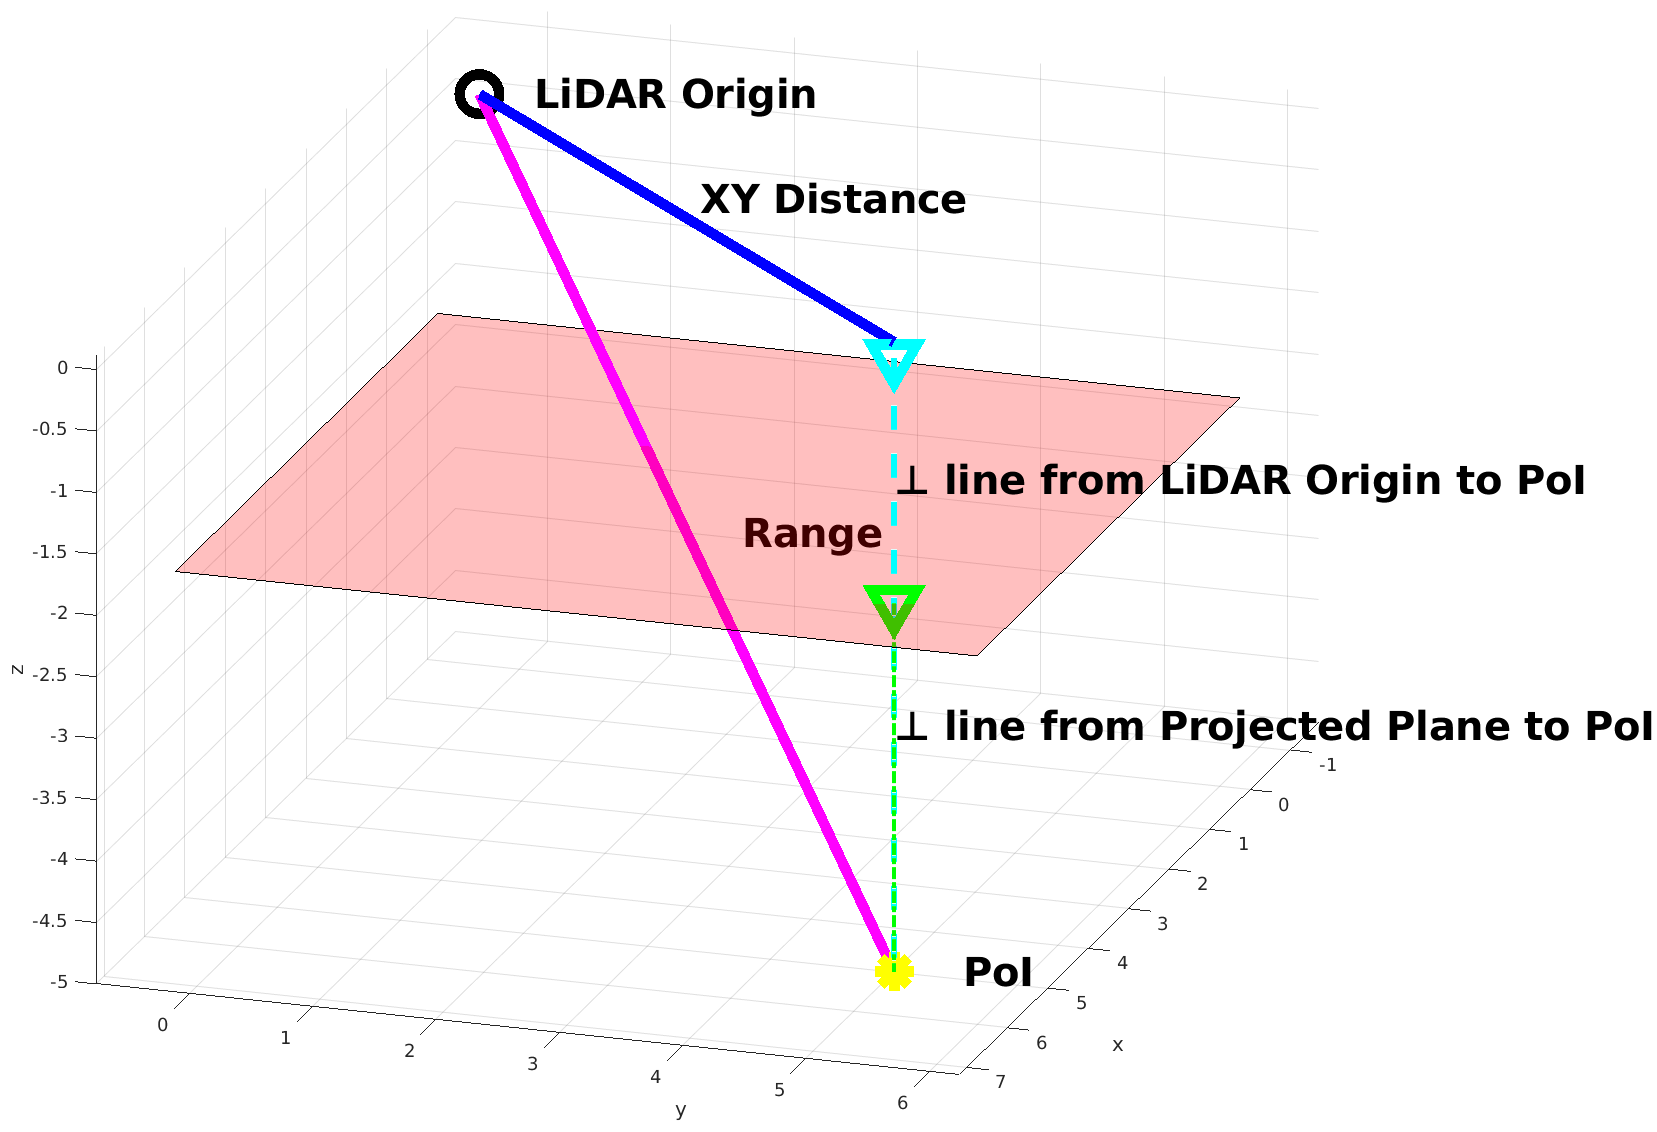
\includegraphics[width=0.5\linewidth]{figures/xy_vs_range}
		\caption[XY vs Range vs Z Height]{Three references for feature extraction may be seen in this simplified graph. First is the Range shown by the magenta line from the LiDAR origin to the Point of Interest (PoI). Second is the height from  LiDAR origin to the PoI (cyan). Finally, distance from the projected plane (red) to the PoI (green). XY Distance (blue) and Range (magenta) from the sensor was used consider the effect of distance from LiDAR origin to the PoI.}
		\label{fig:xy_vs_range}
	\end{figure}
	
	{Feature extraction was completed by performing mathematical functions on the gathered spatial and remission training data. Reference plane normal vector and distance from origin $[a,b,c,d]$ data derived from either RANSAC or Method of Least Squares methods was selected. Base-line features extracted include the following: Standard Deviation ($\sigma$), Roughness ($max - min$), Min-Max Ratio ($min / max$), Min$^{2}$-Max Ratio ($min^2 / max$), and Gradient ($sqrt(\sum_{1}^{n} G))$), where $G$ is an $1*n$ array comprising of the differences between consecutive points in the spatial or remission data array. Distance from the LiDAR point of origin was also considered by dividing the base-line features by either the average range or X-Y distances for a set of points, as LiDAR accuracy may decrease as distance increases. Sixty features were considered in total for this work, and multiple feature sub-sets were used to create a variety of Random Decision Forests. Plane-projection based algorithms were created considering all features. Determination of feature usage allowed for creation of RDFs that used only the top twenty features. Non-plane projection based algorithms were created considering only range and Z height features. For all RDFs, both spatial and remission features were used. } 
	
	{Random Decision Forests were created using MATLAB's $TreeBagger$ function, which creates an ensemble of bagged decision trees using the input arguments of included features, tree depth, number of trees, and a cost array. RDFs were split into sub categories within each feature set to test varying tree depths (Figure \ref{fig:all_tree_comp}), and allowed to grow in number of trees until three hundred trees were created. Discouragement of false-positive identification for road surfaces (gravel and chipseal) was accomplished by introducing a cost array which would induce a bias against gravel and chipseal . Validation error was used as the primary means to compare RDF performance prior to testing with data outside the training and validation data sets. MATLAB was used to load verification data and test increasing sizes of RDF algorithms for accuracy by comparing the known data types against the RDF result. Plotting number of trees verses error allowed for determination of an early stopping point for algorithm growth (Figure \ref{fig:mls_zxy_early_stopping}) by choosing the point where the change in error moving average did not exceed 10\% and was within 20\% of the minimum error.}
	
	\begin{figure}[H]
		\centering
		\begin{subfigure}{0.45\textwidth}
			\centering
			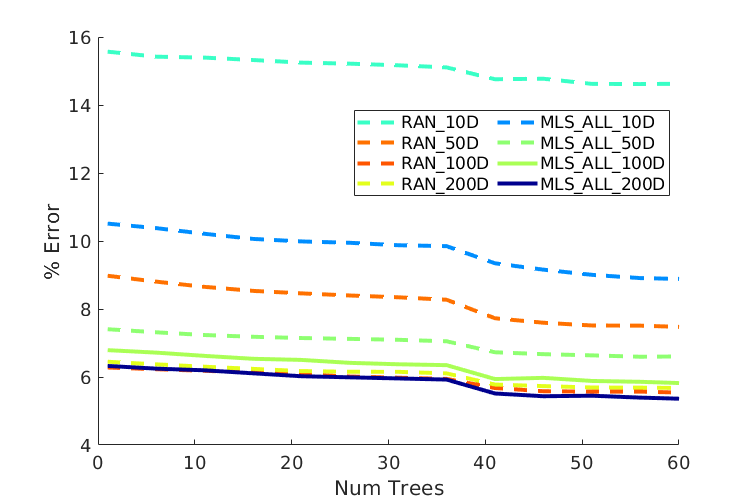
\includegraphics[width=1\linewidth]{figures/MLS_RAN_ALL}
			\caption[]{}
			\label{fig:all_mls_ransac_comp}
		\end{subfigure}
		\begin{subfigure}{0.45\textwidth}
			\centering
			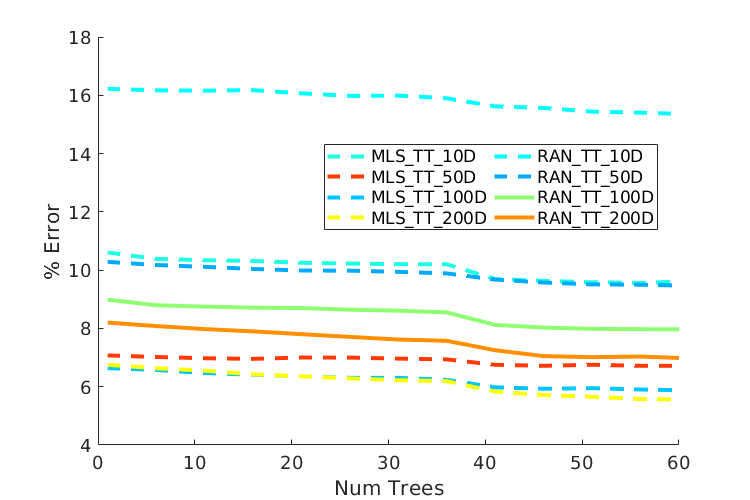
\includegraphics[width=1\linewidth]{figures/MLS_RAN_TT}
			\caption[]{}
			\label{fig:xyz_mls_ransac_comp}
		\end{subfigure}
		\label{fig:xyz_mls_comp_1}
		\begin{subfigure}{0.45\textwidth}
			\centering
			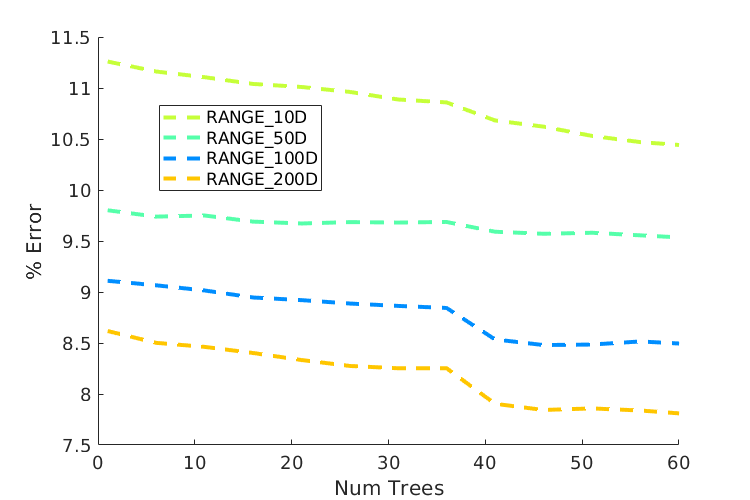
\includegraphics[width=1\linewidth]{figures/Range_Vali_Error}
			\caption[]{}
			\label{fig:range_mls_ransac_comp}
		\end{subfigure}
		\begin{subfigure}{0.45\textwidth}
			\centering
			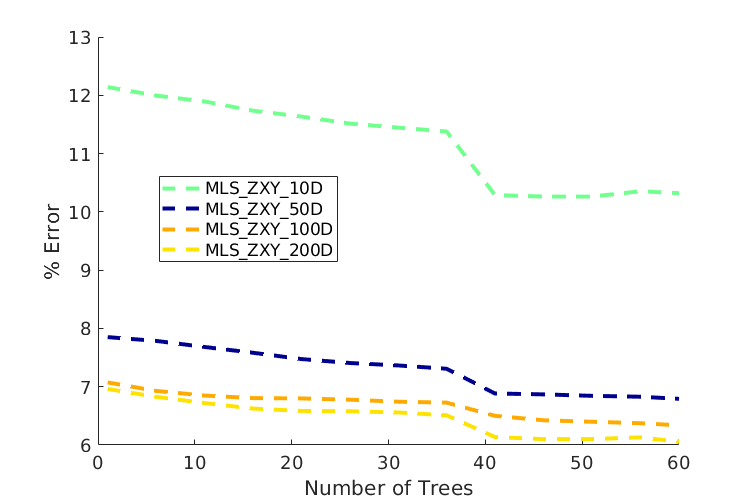
\includegraphics[width=1\linewidth]{figures/ZXY}
			\caption[]{}
			\label{fig:t20_mls_ransac_comp}
		\end{subfigure}
		\caption[RDF Validation Accuracy]{RDF validation accuracy directly compared. All features are considered (a); Top 20 features used in (a) only (b); Range was used without X, Y, and Z components broken out (c); Plane projection not considered in (d), reference plane set as the LiDAR origin point.}
		\label{fig:all_tree_comp}
	\end{figure}

	\begin{figure}[H]
			\centering
			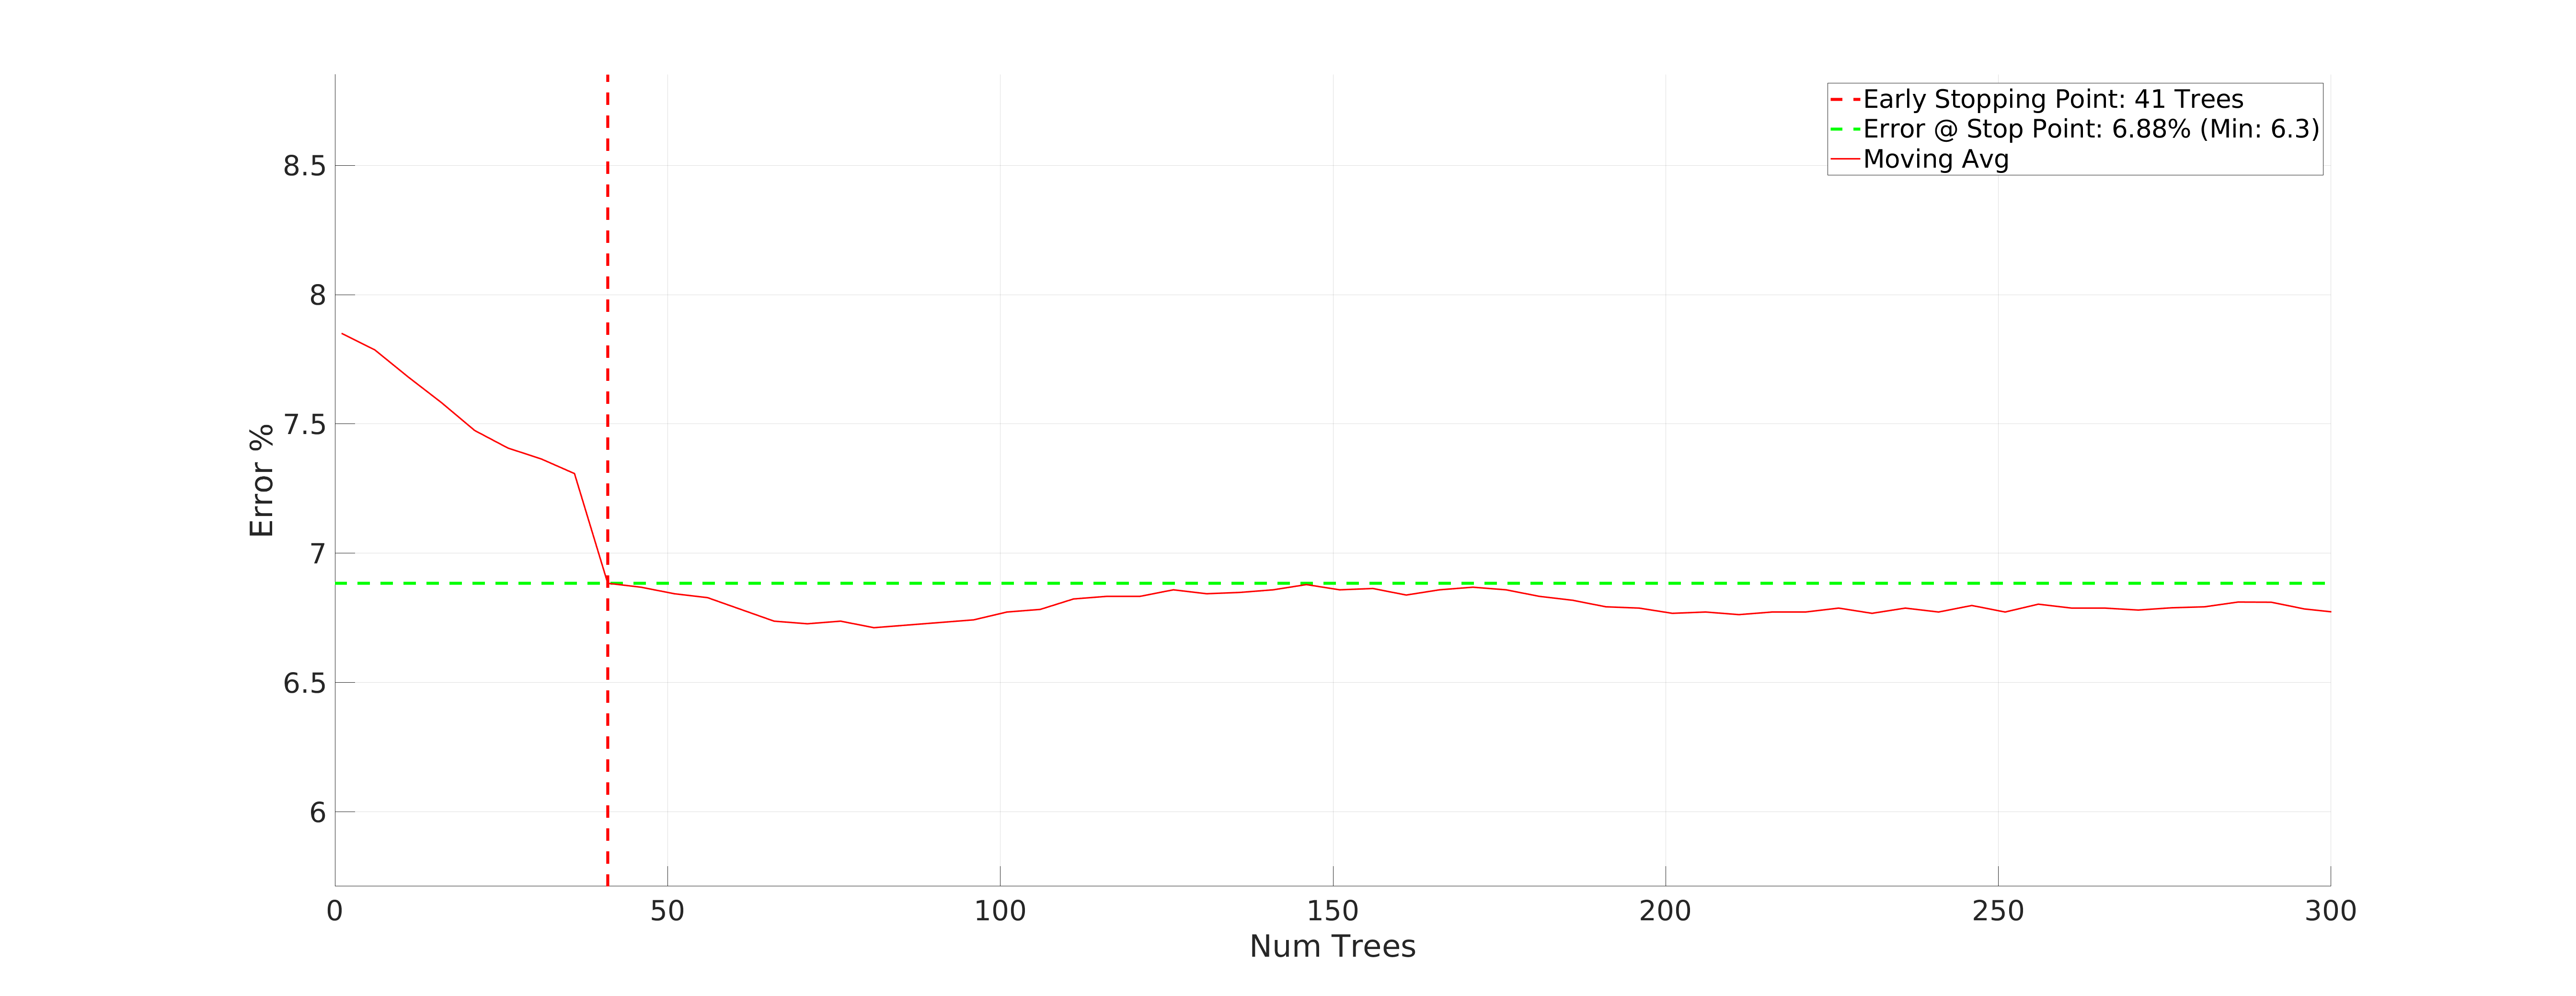
\includegraphics[width=0.75\linewidth]{figures/mls_zxy_early_stopping}
			\caption[Early Stopping]{Diminishing returns on increasing algorithm size versus accuracy can be used to determine the early stopping point of algorithm growth.}
			\label{fig:mls_zxy_early_stopping}
	\end{figure}
	
	% Quadrant size inversely affects rate of classification, as smaller quadrants allow for greater resolution at the expense of more computational time. 
	
	{Testing consecutive scans required a method of compiling LiDAR data into a single point cloud and manually classifying areas for road detection accuracy, completed by post processing rosbags that contained scanning LiDAR, GPS, and IMU data of an unmarked road. Point cloud translation and rotation was accomplished using transformation matrices derived from GPS and IMU data. Rotation matrices were created using extracted roll, pitch, and yaw data from the IMU. LiDAR origin was found using GPS longitude, latitude, and altitude data. Physical distances between the GPS, IMU, and LiDAR was rectitude by obtaining reference frames provided by AutonomouStuff. GPS coordinates were offset by the current orientation and converts the ground truth to the LiDAR frame. GPS, IMU, and LiDAR reference frames and rotational updates were combined into trajectory vectors. Consecutive point cloud scans may then translated and rotated with derived transformation matrices (Figure \ref{fig:Compiled_PCD}). While not as robust as more sophisticated methods of point cloud aggregation such as NDT or ICP scan matching, over shorter distances using this method proved to be adequate for scoring purposes. Six stretches of unmarked roads were examined for accuracy: three of chipseal and three of gravel. Road and side-of-road areas were manually defined and projected unto consecutive LiDAR scans to score classification results. Due to the fuzzy nature of the classification results, the side-of-road areas were roughly a standard lane width to the sides of the road to accommodate the inability to define a ridge road edge.}
	
	\begin{figure}[H]
		\centering
		\begin{subfigure}{0.45\textwidth}
			\centering
			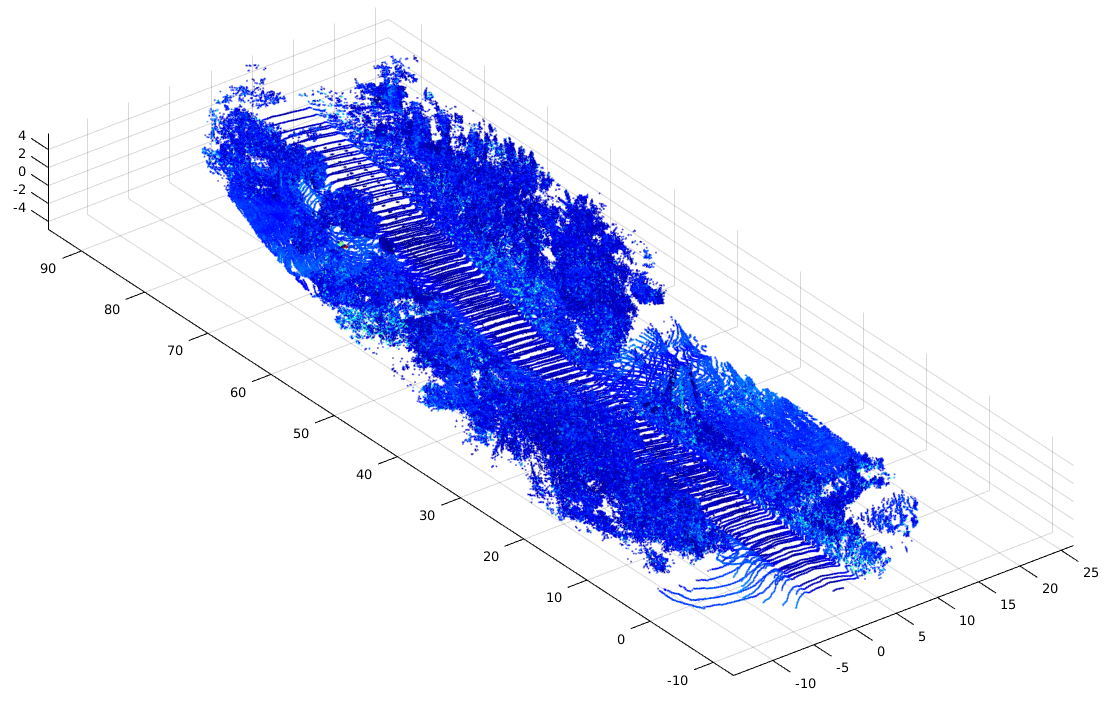
\includegraphics[width=0.95\linewidth]{figures/Compiled_PCD}
			\caption[C]{}
			\label{fig:Compiled_PCD}
		\end{subfigure}
		\begin{subfigure}{0.45\textwidth}
			\centering
			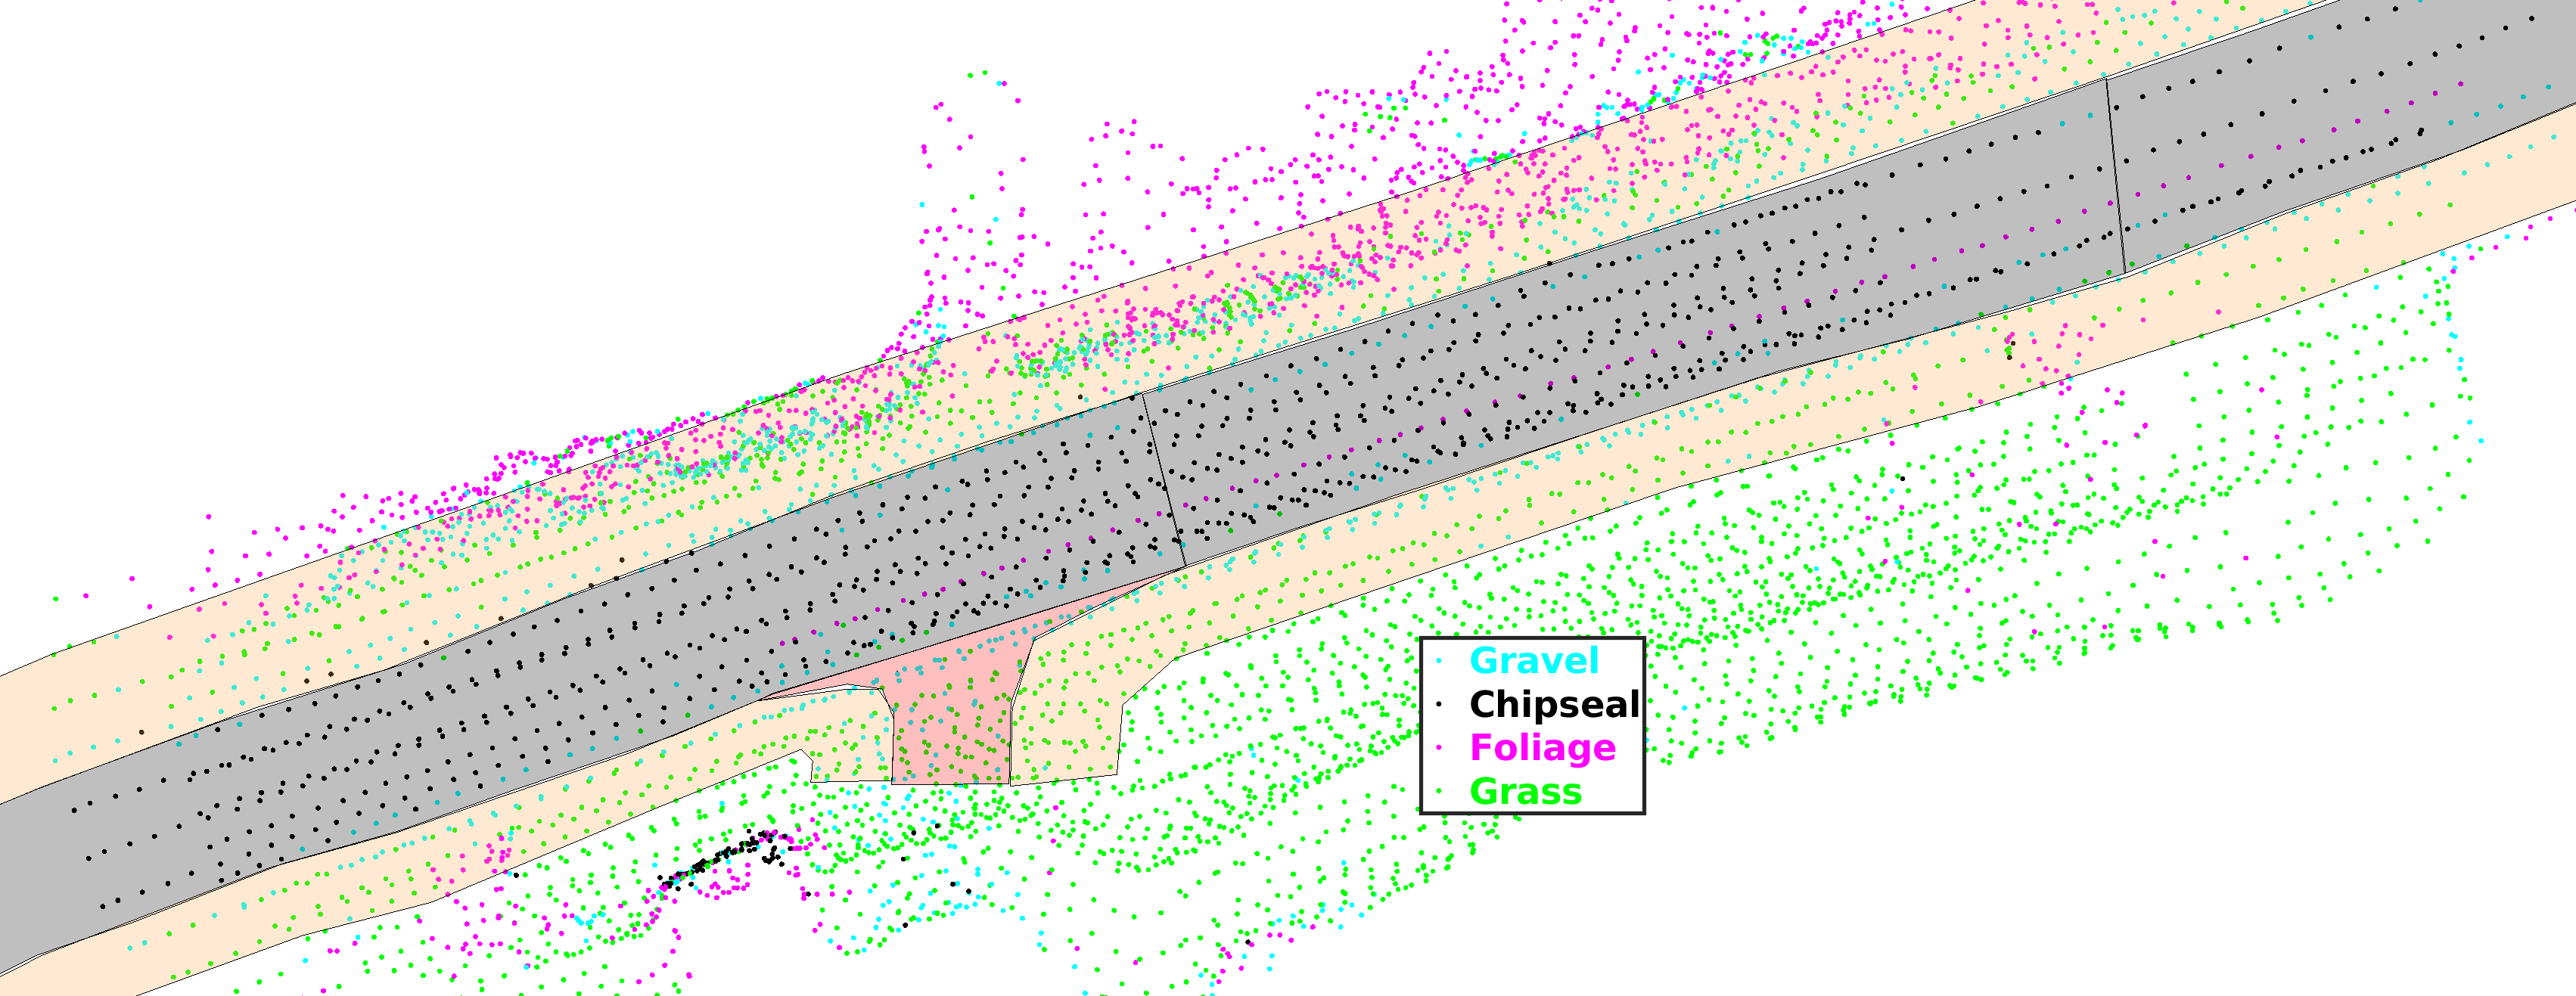
\includegraphics[width=0.95\linewidth]{figures/short_chip_redux}
			\caption[]{}
			\label{fig:Classified_Areas_PCD}
		\end{subfigure}
		\caption[Compiled and Classified Point Cloud Data]{Point cloud of scanning LiDAR data using GPS and IMU data to determine point of origin and orientation for the LiDAR (a). Point cloud data was classified, and then scored using manually defined road and side-of-road areas (b).}
		\label{fig:Combined_Classified_PCD}
	\end{figure}
	
	{Classifying gathered consecutive LiDAR scans was accomplished by analyzing each individual 360$^{\circ}$ sweep of the discretized channels. Each channel was broken into quadrants. Quadrant size inversely affects rate of classification, as smaller quadrants allow for greater resolution at the expense of more computational time. Translation and rotation was applied to the terrain classification results with the closest matching transformation matrices.Classification results that were sympatric to manually defined areas were examined for accuracy by scoring the exact terrain classification and true/false-positive road surface detection. Drop off in positive road surface classification rates in side-of-road areas in side-of-road areas would be indicative of adequate road edge detection. Consecutive scanning LiDAR data was compiled allowing for manually assigning areas representing road or side of road surfaces (Figure \ref{fig:Classified_Areas_PCD}).}
	
%	{ Comparing averaged X, Y, and Z coordinates of the classified quadrant allowed for easier comparison and scoring of the RDF classification to the manually classified areas. 
% Insert sentence or two on rate of of classification, feat extract, etc.; reference figure with rates> This was tested with a machine with 64 GB of DDR4 RAM and a Ryzen 9 5900X 12 core x 24 thread CPU.}
	
\section{Results}
	
	{Scanning LiDAR, GPS, and IMU data was collected on closed lots and public roads near Athens Ohio using the Experimental Apparatus. Gravel and chipseal data was gathered from closed lots and unmarked public roads (Figures \ref{fig:Combined_Roads}), while grass (well-trimmed lawn grass) and foliage (leafy trees and bushes) was gathered from areas surrounding public roads. Training data was generated using MATLAB to extract LiDAR data from rosbags. Classification algorithms using Random Decision Forests were generated using a variety of feature sets and reference points. Testing consecutive scans was completed by post processing rosbags that contained scanning LiDAR, GPS, and IMU data. Physical distances between the GPS, IMU, and LiDAR were rectified by measuring the distance between the modules. Rotational reference frames between the GPS, IMU, and LiDAR were rectified by applying appropriate rotational matrices. Transformation matrices were created by considering the GPS position and the IMU's roll, pitch, and yaw data. Point cloud data was then classified using the RDF derived in Objective I. Translation and rotation was applied to the terrain classification results. Consecutive scanning LiDAR data was compiled allowing for manually assigning areas representing road or side of road surfaces (Figure \ref{fig:classified_point_clouds_all}). Side of road area were manually defined as an area roughly one meter outwards from the road edge for consideration of road edge detection.}
		
	\begin{figure}[H]
		\centering
		
		\begin{subfigure}{0.495\textwidth}
			\centering
			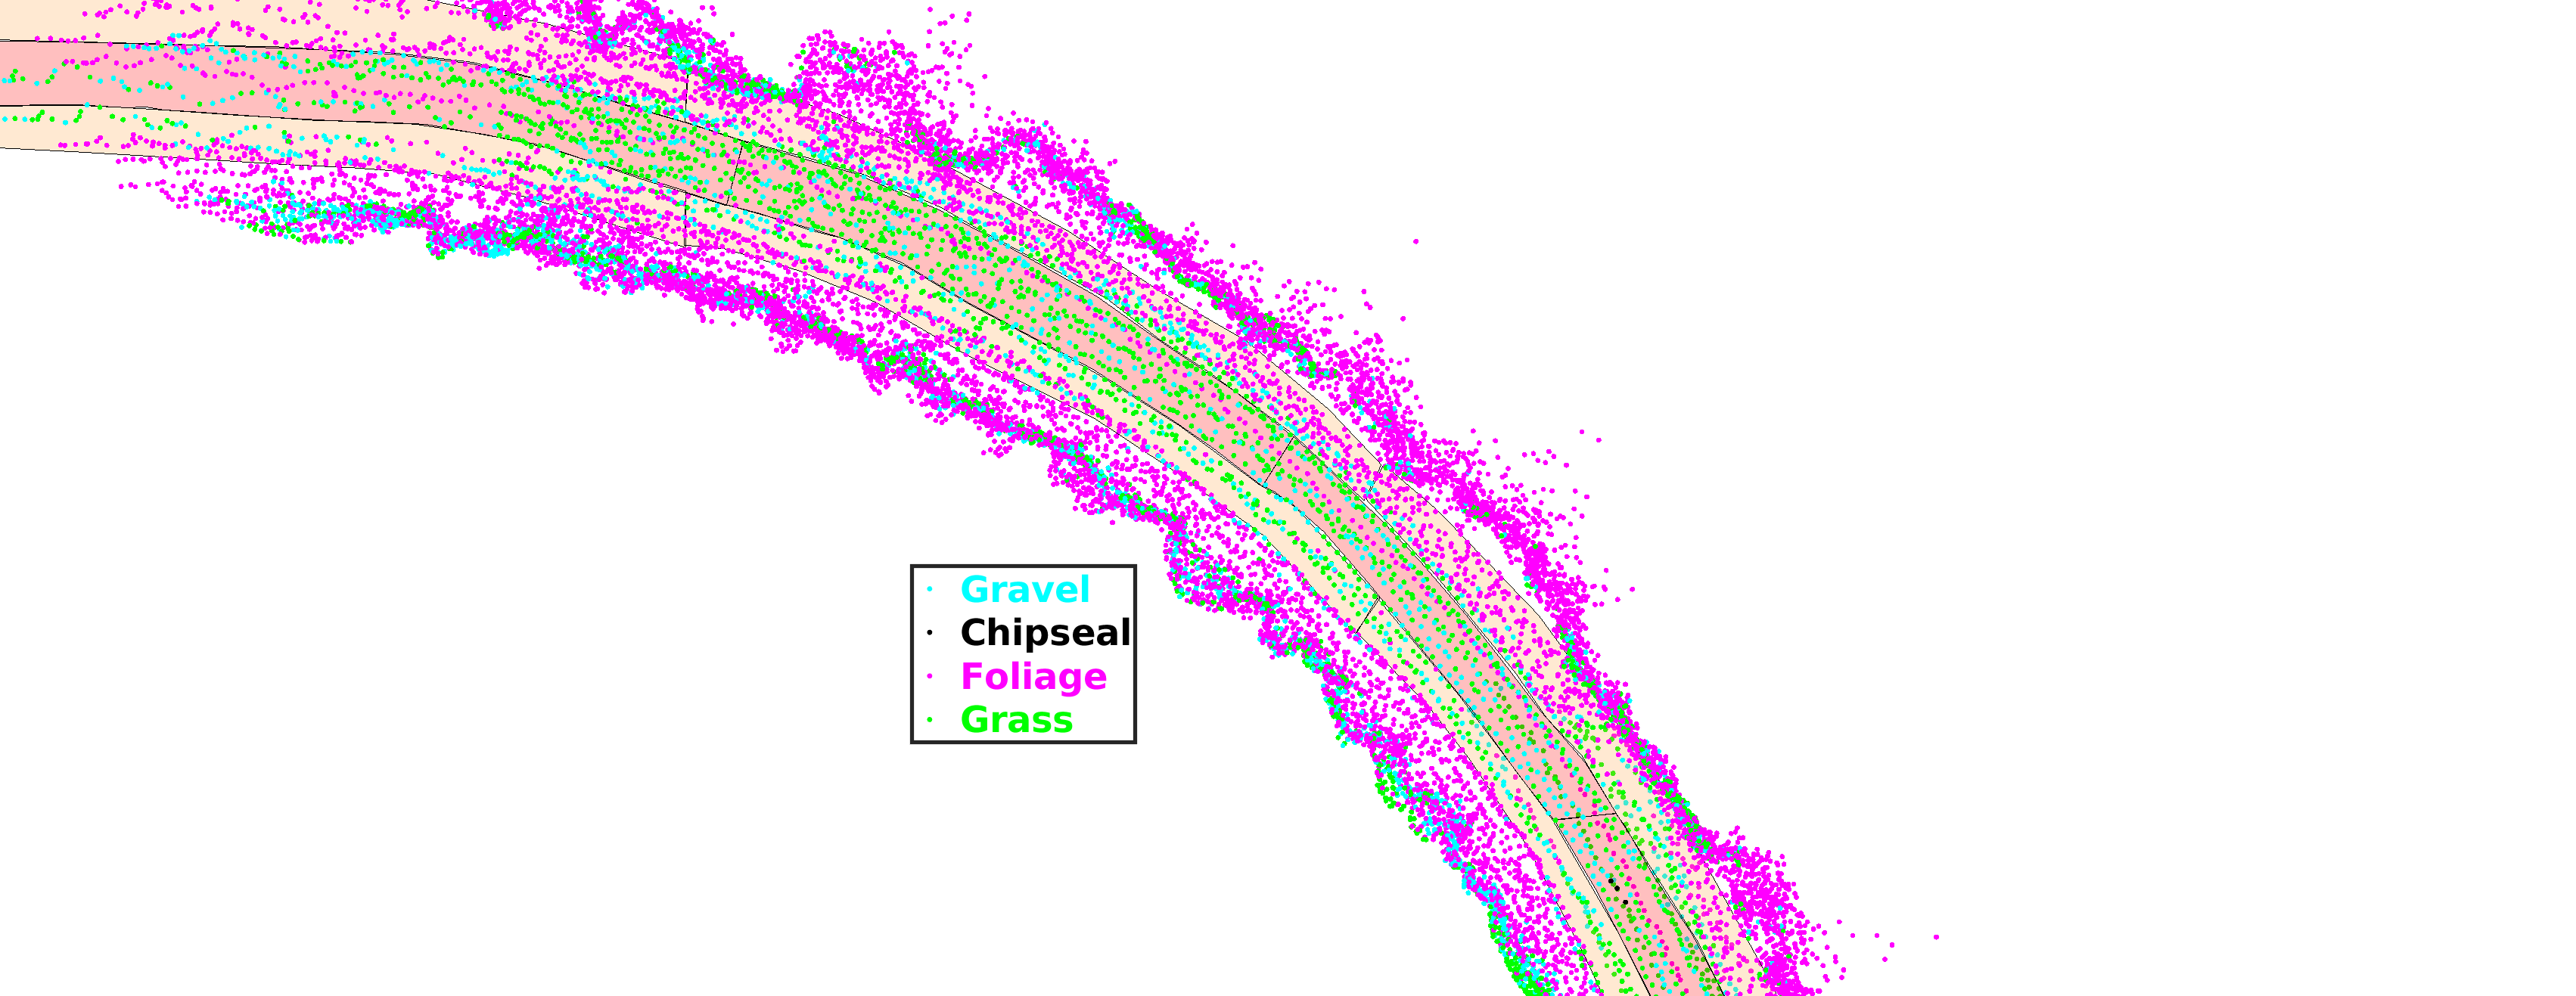
\includegraphics[width=0.95\linewidth]{figures/curve_gravel}
			\caption[]{}
			\label{fig:curve_gravel_2}	
		\end{subfigure}
		\begin{subfigure}{0.495\textwidth}
			\centering
			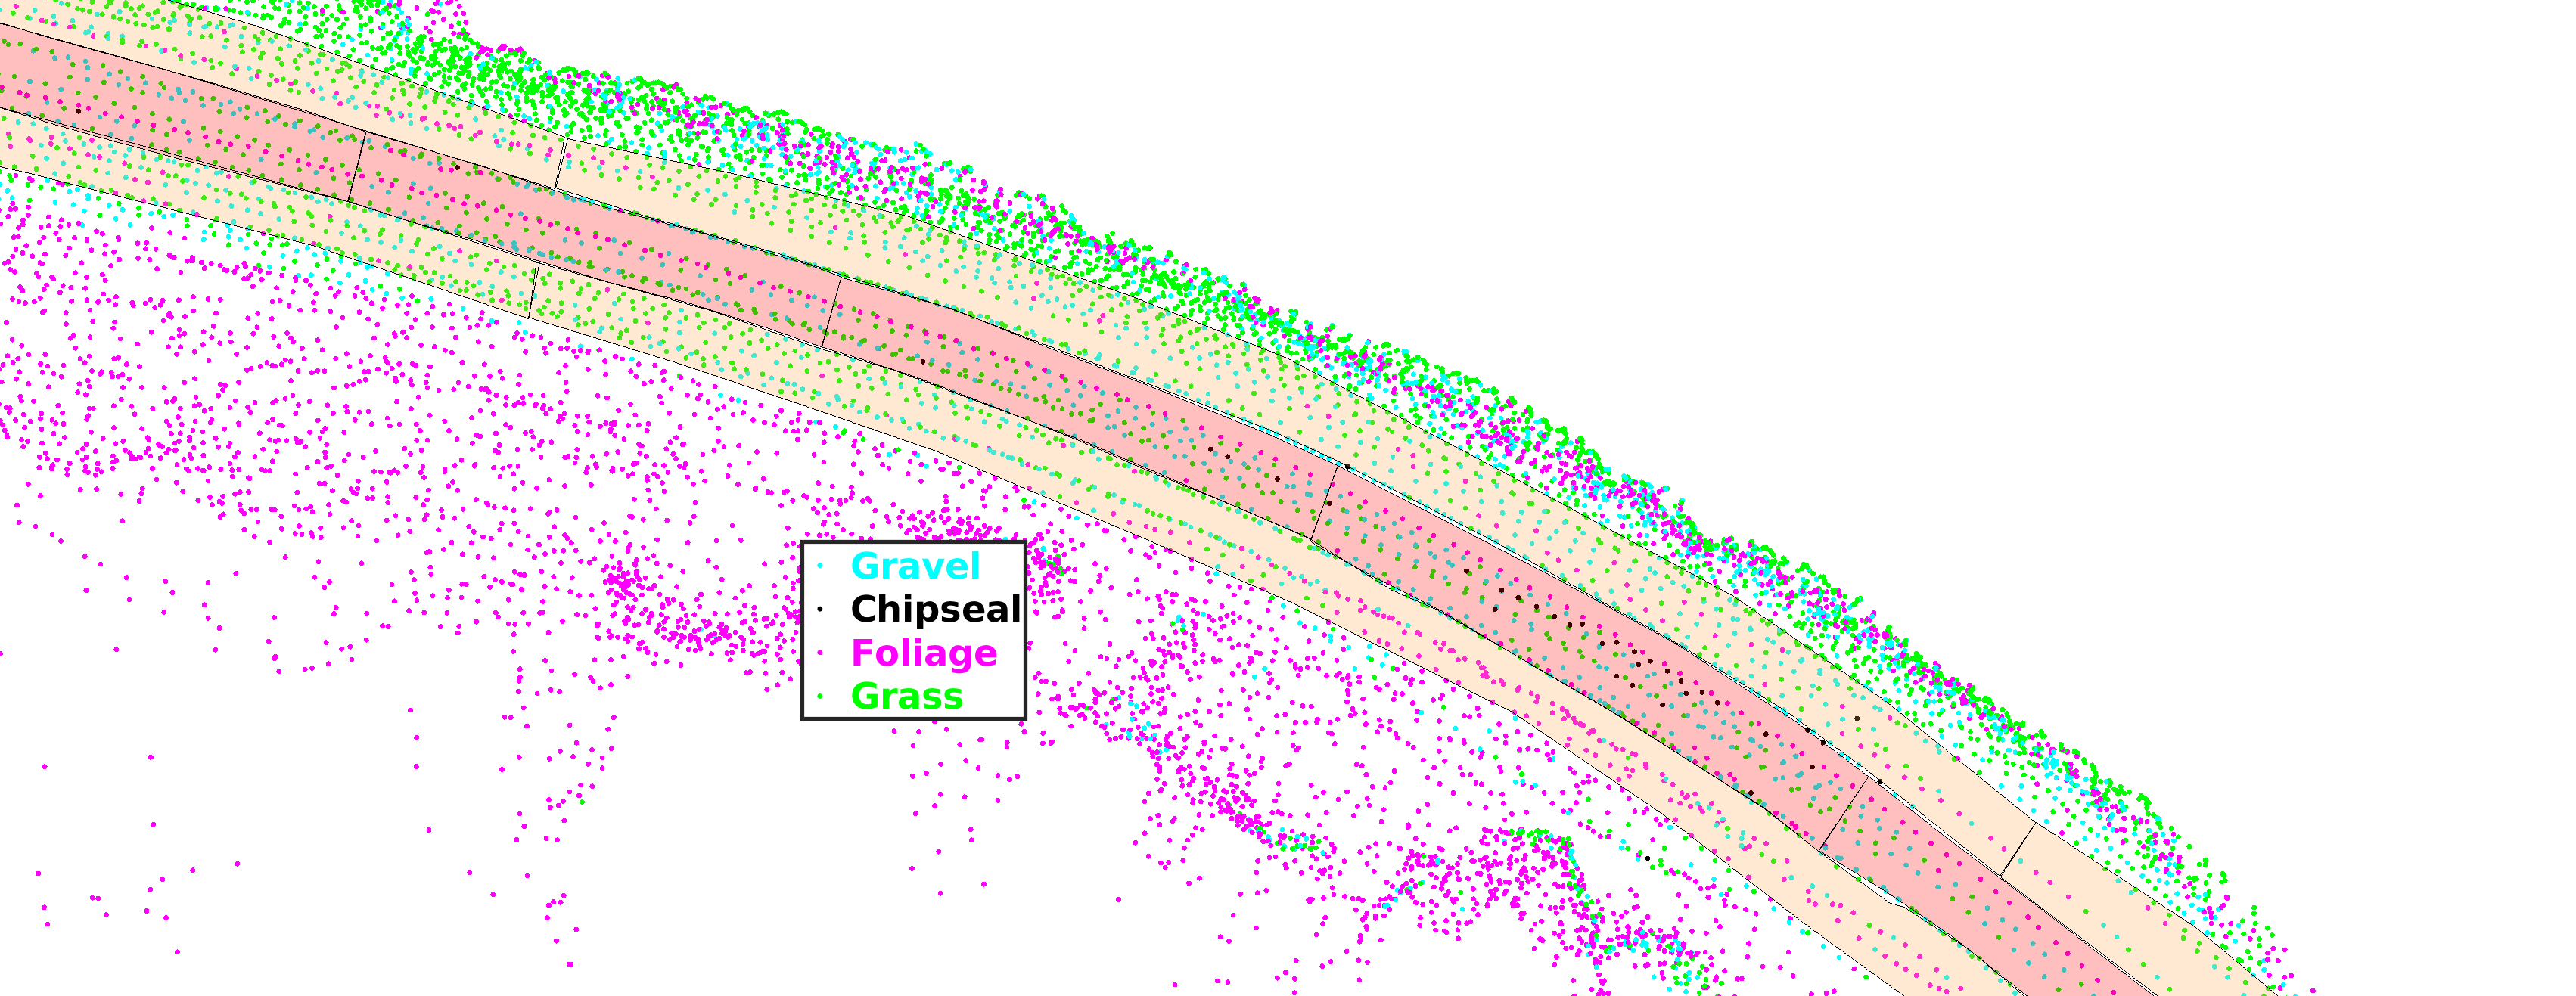
\includegraphics[width=0.95\linewidth]{figures/curve_gravel_2}
			\caption[]{}
			\label{fig:curve_gravel}
		\end{subfigure}
		\begin{subfigure}{0.495\textwidth}
			\centering
			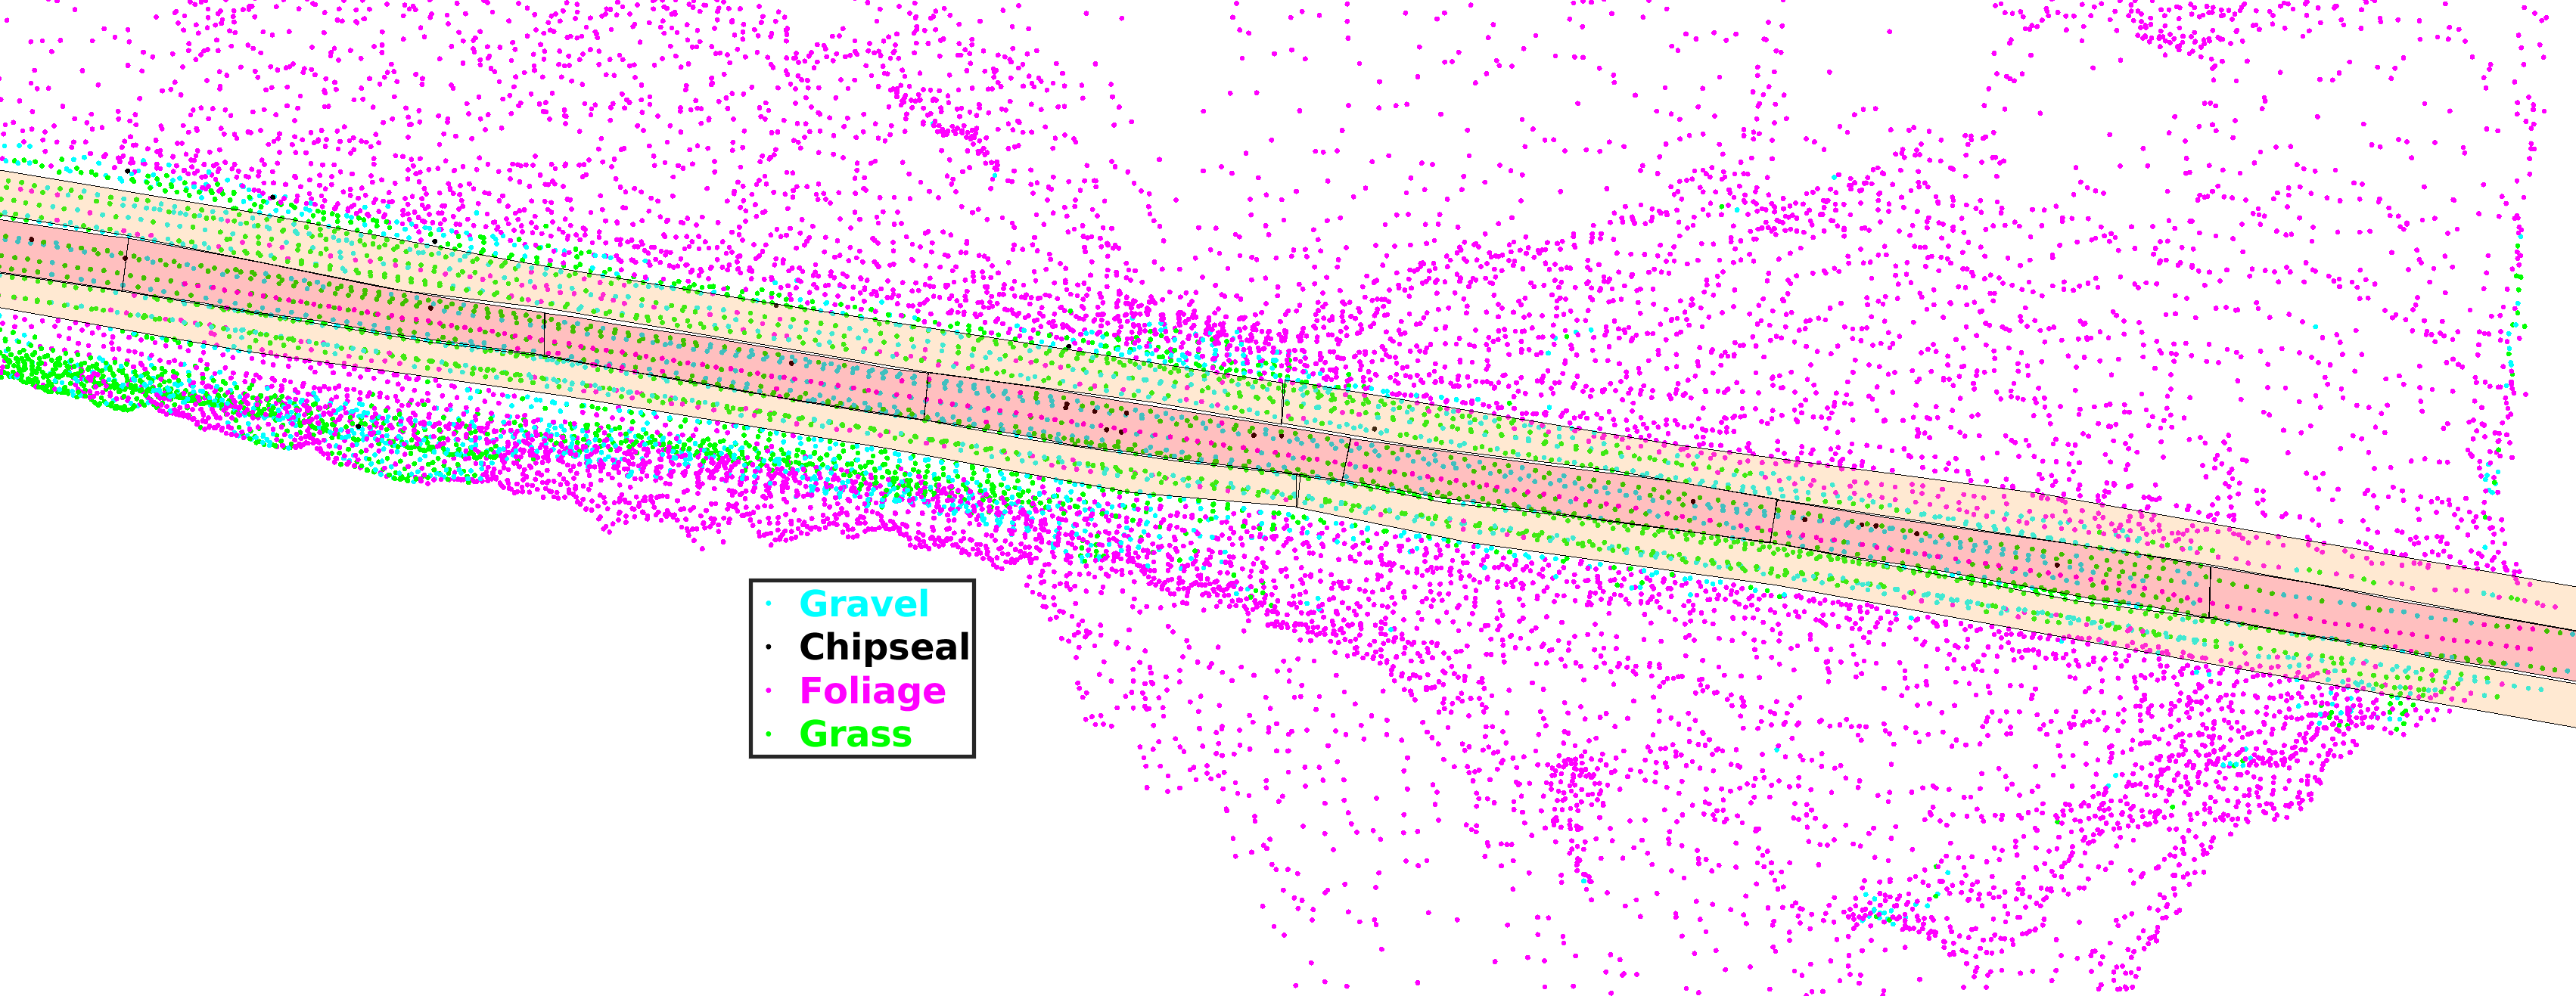
\includegraphics[width=0.95\linewidth]{figures/long_gravel_1}
			\caption[]{}
			\label{fig:long_gravel_1}	
		\end{subfigure}
		\begin{subfigure}{0.495\textwidth}
			\centering
			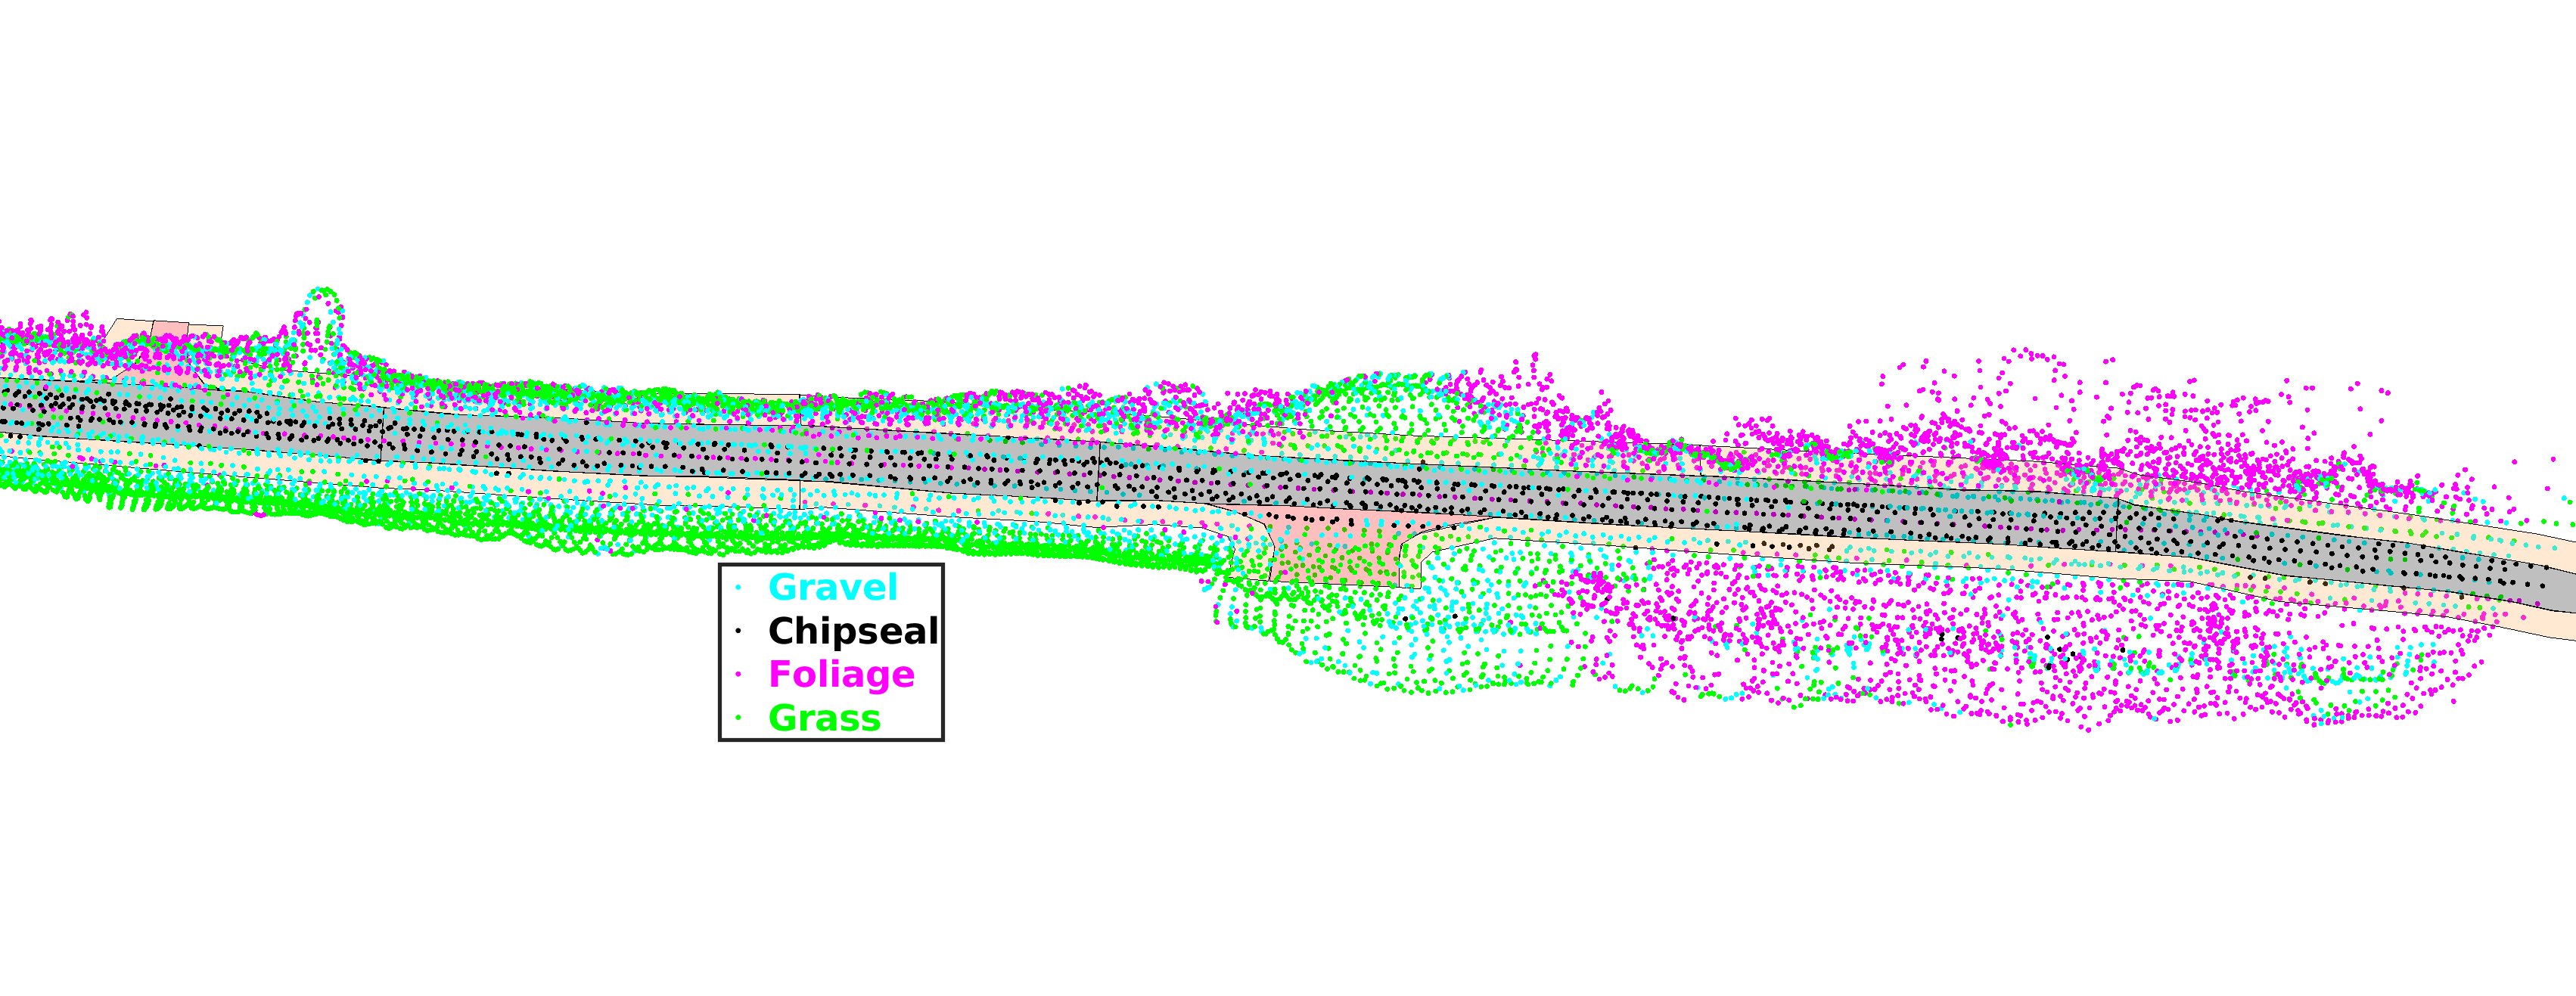
\includegraphics[width=0.95\linewidth]{figures/long_chip_redux}
			\caption[]{}
			\label{fig:long_chip_classified}
		\end{subfigure}
		\begin{subfigure}{0.495\textwidth}
			\centering
			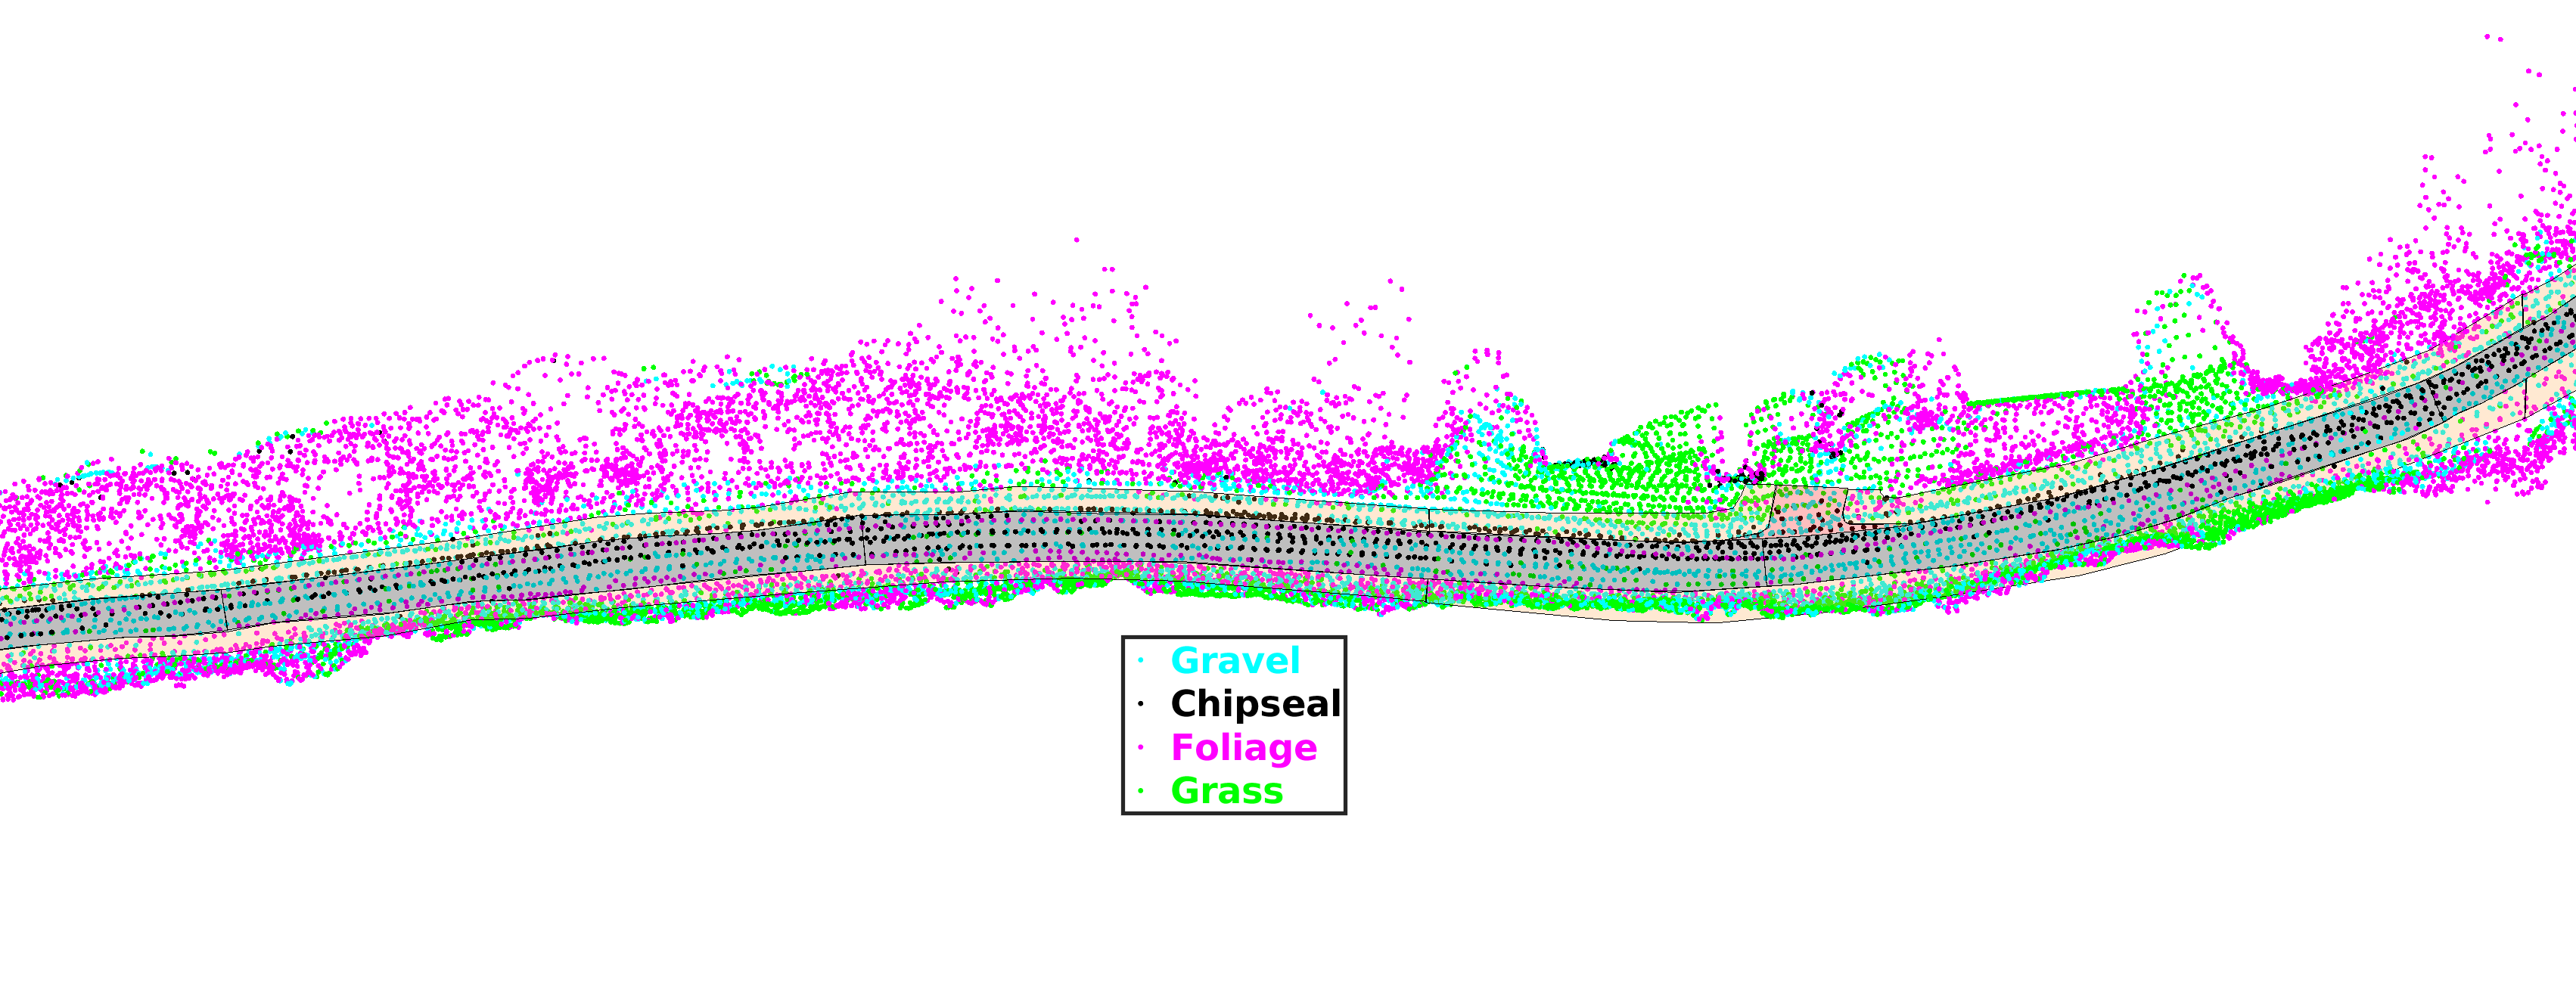
\includegraphics[width=0.95\linewidth]{figures/long_chip_redux_2}
			\caption[]{}
			\label{fig:long_chip_2_classified}
		\end{subfigure}
		\begin{subfigure}{0.495\textwidth}
			\centering
			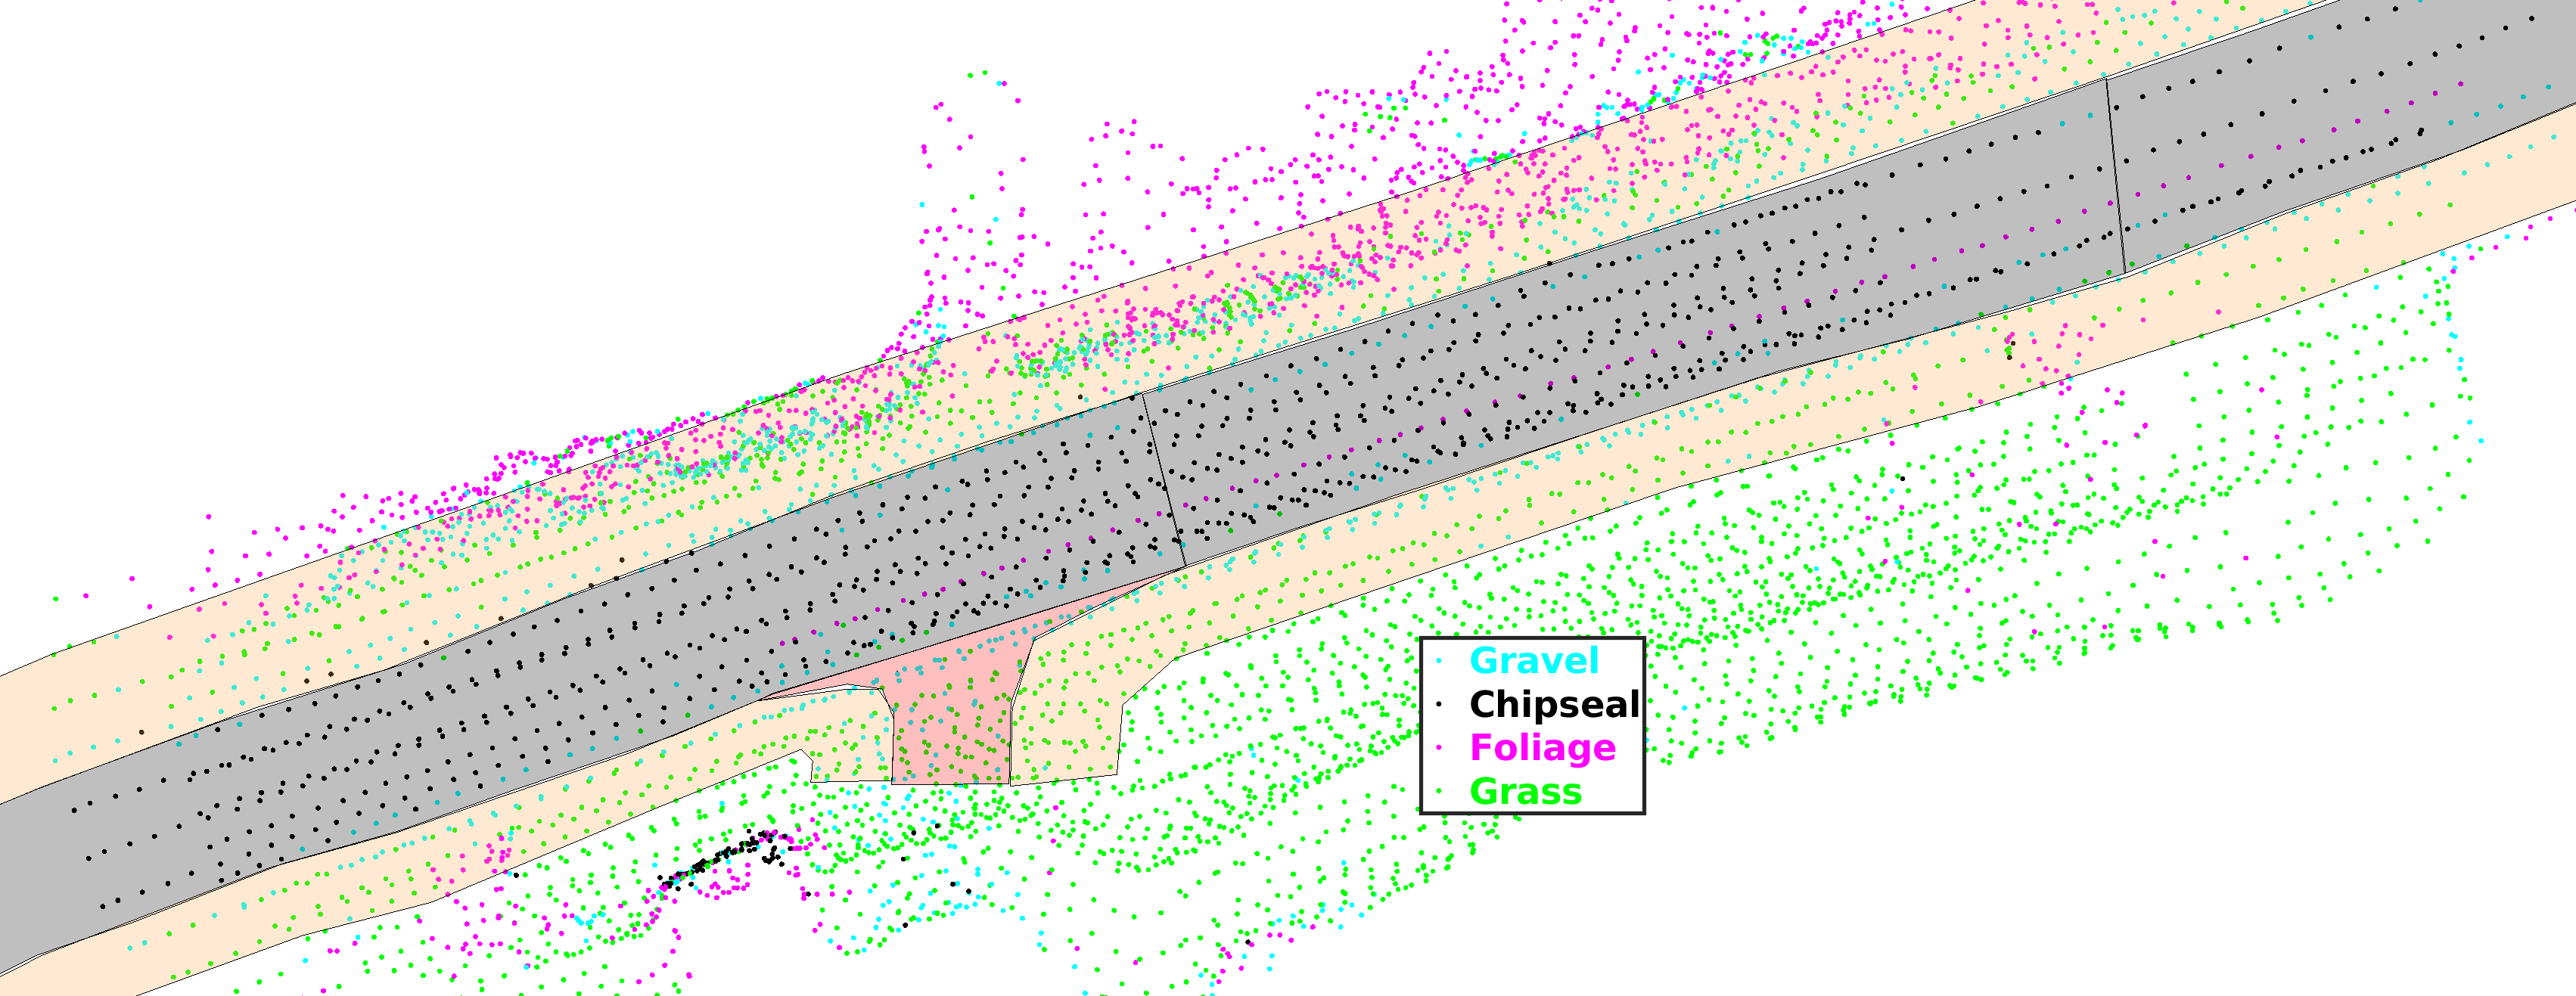
\includegraphics[width=0.95\linewidth]{figures/short_chip_redux}
			\caption[]{}
			\label{fig:short_chip_classified}
		\end{subfigure}
		\caption[Classified Point Clouds]{Classified point clouds with manually defined surface areas that allow for scoring of classification results. Gravel roads include an un-named gravel side-road near Armig Road (a) and Sturbois Road (b), (c). Chipseal roads include Willow Creek Road (d), (e), and Bean Hollow Road (f). The algorithm that produced these results used all features and reference plane projected with RANSAC. Chipseal roads are shown as black areas, gravel roads and driveways are shown as red areas, and side-of-roads are designated as orange. }
		\label{fig:classified_point_clouds_all}
	\end{figure}

	{Results were scored by comparing the location of the averaged classified quadrant's (x,y) coordinate to the area that the manually defined areas (Table \ref{tab:averaged_results} shows results for algorithm designation RAN ALL which produced the results in Figure \ref{fig:classified_point_clouds_all}. All results are shown in Table \ref{tab:all_results} in Appendix \ref{apdx:Appendix_2}). Ratio of road to non-road in manually defined road and side-of-road areas are shown in columns 3 and 4, with higher values indicating a greater presence of positive road identification. The quotient of the two ratios (col. 5) allows for estimation of road edge detection ability. Scores for correct and incorrect road surface type is shown, indicating the algorithm's ability to correctly determine the road surface type (cols. 6,7). Percentages of grass and foliage classification for both side-of-road and on road are given in cols. 8 \& 9, indicating true/false-negative road surface identification capability. True/false-positive road surface identification percentages are indicated in cols 10-11.}

	{It was found that while none of the algorithms excelled in all areas, the results seem to indicate that implementing a multiple-model algorithm to create an ensemble would greatly increase road detection accuracy. Of the algorithms tested (Appendix \ref{apdx:Appendix_2}), the RDF that used RANSAC as the plane projection method and the full feature (designated RAN ALL) performed the most consistently for true non-road surface identification, with an average of 66.5\% (median of 65.5\%). While it did struggle with gravel identification (32.72\% average accuracy) with a high confusion rate with grass (27.47\% false identification), it may be supplemented with the RDF designated RANGE, which has the highest true-positive gravel identification rate of 82.8\%. A classification method was tested to verify this method based on RAN ALL and RANGE algorithms. RAN ALL would would designate non-road surfaces and the determination of road surface type was a combined effort of the two (Figure \ref{}), thus achieving a higher accuracy. }
	
	\begin{table}[H]
		\centering
		\begin{tblr}{width=0.9\linewidth,colspec={|Q[1,m,c]|Q[1.5,m,c]|Q[1.5,m,c]|Q[1.5,m,c]|Q[1.5,m,c]|Q[1.5,m,c]|}}
			\hline
			Algorithm Designation & Average \% of True Gravel Type Identification & Average \% of True Chipseal Type Identification & Average \% of True Surface Type Identification & Average \% True Road Surface Detection & Average \% of True  Non-Road Surface Detection\\
			\hline
			MLS ALL & 35.354 & 68.581 & 46.587 & 82.896 & 55.006 \\
			\hline
			MLS TT  & 37.833 & 55.162 & 40.865 & 89.444 & 37.308 \\
			\hline
			ZXY     & 35.697 & 73.211 & 50.601 & 93.153 & 55.156 \\
			\hline
			RAN ALL & 36.119 & 54.169 & 42.376 & 56.252 & 66.500 \\
			\hline
			RANGE   & 61.822 & 44.758 & 51.610 & 78.526 & 47.918 \\
			\hline
			RAN TT  & 54.508 & 27.617 & 57.293 & 65.323 & 58.506 \\
			\hline
%			Ens\_1  & 61.822 & 44.758 & 51.610 & 78.526 & 66.685 \\
%			\hline
		\end{tblr}
		\caption[Averaged Results]{Average results of all algorithms on tested roads. }
		\label{tab:averaged_results}
	\end{table}
	
%	\begin{figure}[H]
%		\centering
%		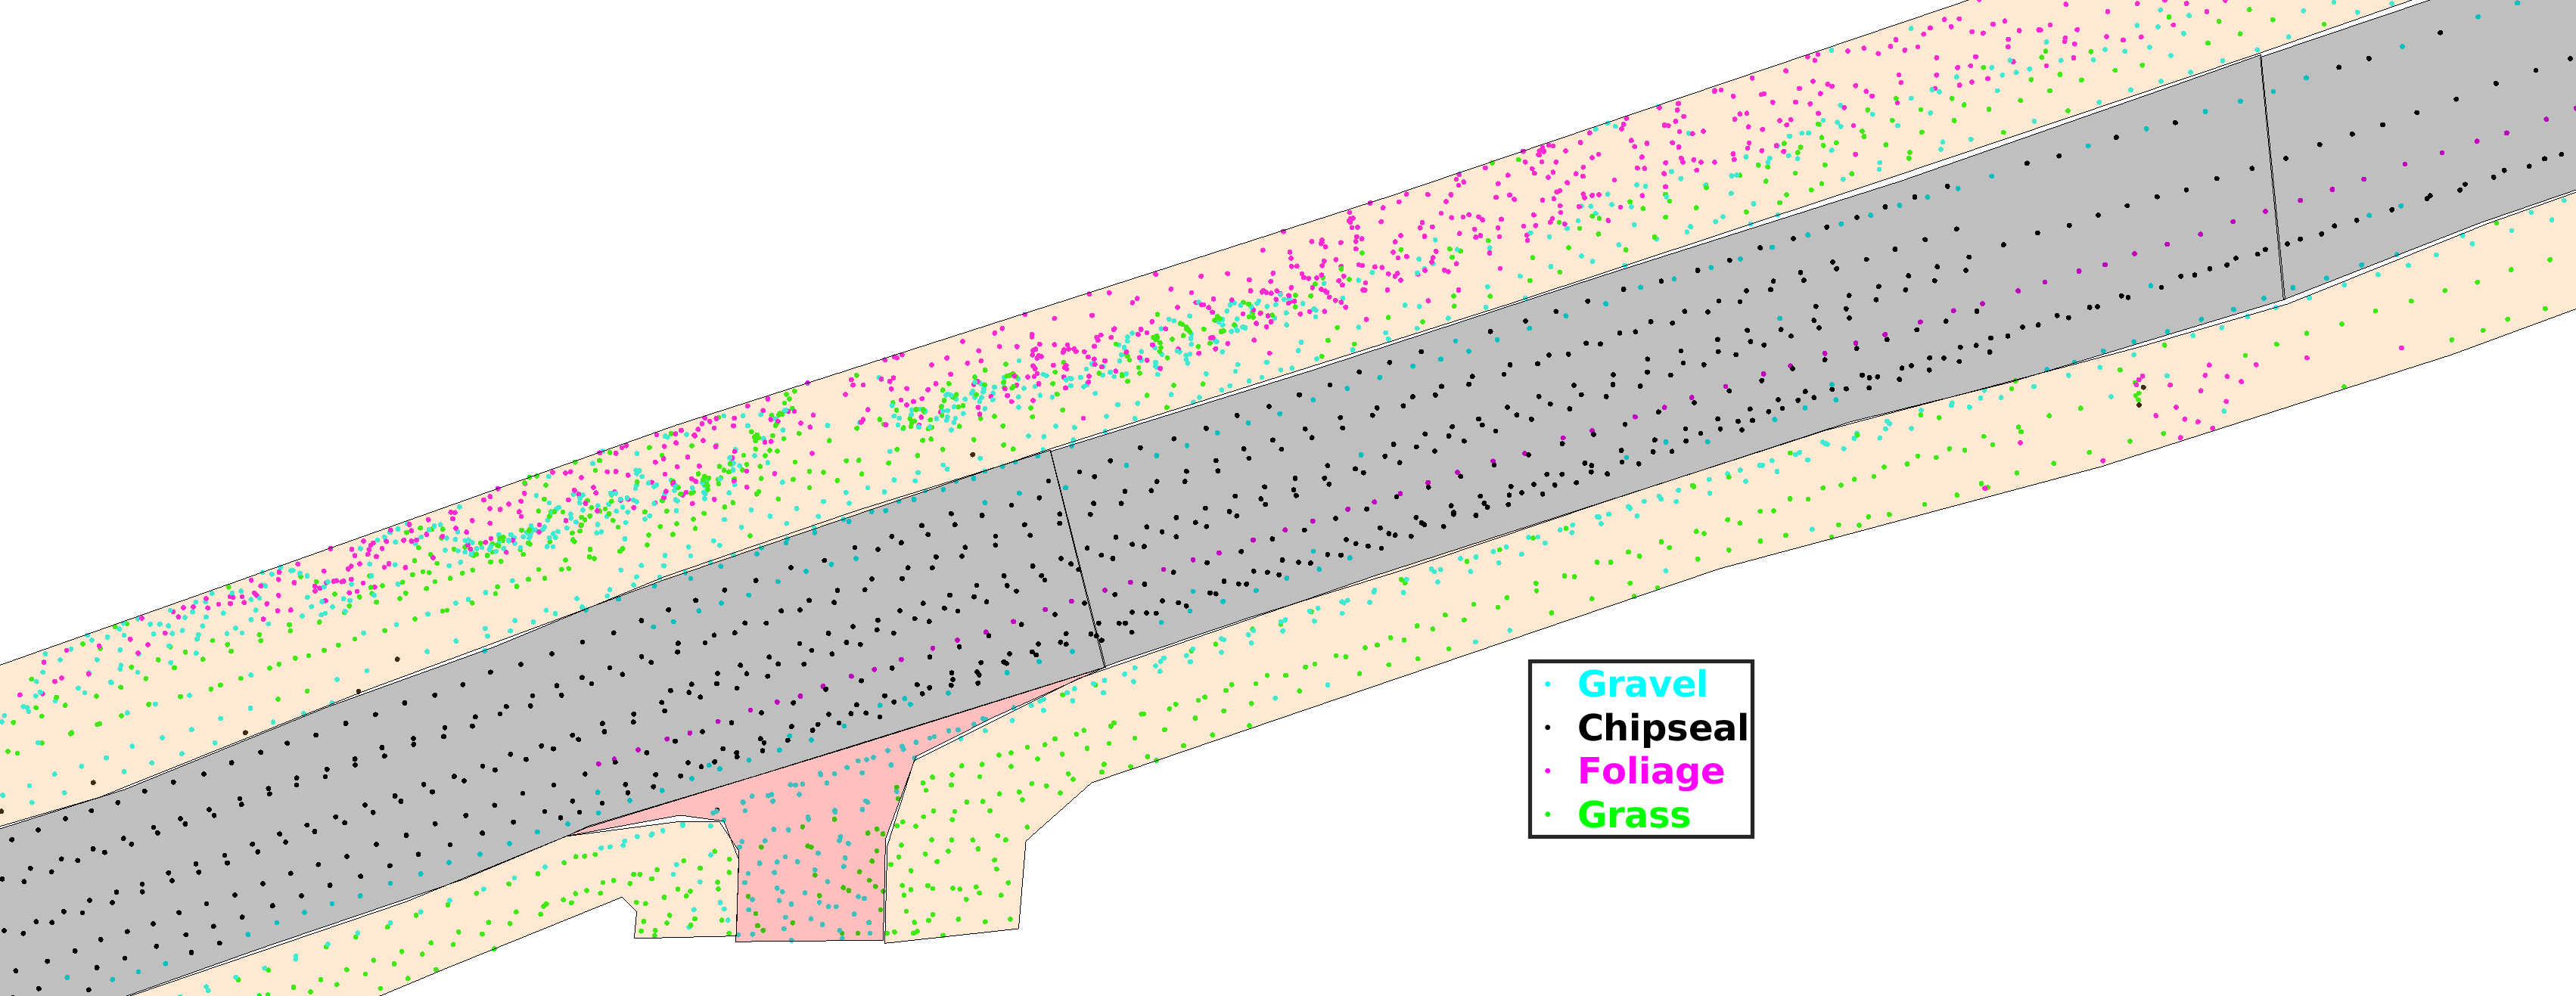
\includegraphics[width=0.75\linewidth]{figures/RAN_ALL_ofroad_RANGE_onroad}
%		\caption[Early Stopping]{Diminishing returns on increasing algorithm size versus accuracy can be used to determine the early stopping point of algorithm growth.}
%		\label{fig:combo_result}
%	\end{figure}	
	
	{Quadrant size affects terrain classification accuracy at the expense of granularity of results and computational time. Smaller quadrants allow for greater resolution of terrain classification, however more computational time is required. Larger quadrants allow for swifter classification, however as consecutive scanning LiDAR points may include road and non-road surfaces, classification accuracy may suffer. Best per-Quadrant average classification rate was X.XX quadrants per second as tested on a machine with 64 GB of DDR4 RAM and a Ryzen 5900x @ 3.70GHz*24.}
	
	


\section{Conclusion}
	
	{The proposed work addresses the problem of road surface detection on unmarked gravel and chipseal roads. Current LiDAR and Camera based detection models are insufficient due to lack of distinct features typical of urban roads, such as painted line markings or curbs, or have excessive computational or storage requirements. The completed work balanced accuracy and efficiency by using less intensive analysis techniques of smaller point cloud data sets. The final deliverable of the described work was a method of detecting physical unmarked gravel and chipseal roads by using a terrain classification approach to predicting road surface area. The impact of this work is that autonomous vehicles using LiDAR may be able to detect unmarked gravel and chipseal road surfaces, allowing autonomous operations on 1.5 million miles of previously undetected rural roads.}


% For peer review papers, you can put extra information on the cover
% page as needed:
% \ifCLASSOPTIONpeerreview
% \begin{center} \bfseries EDICS Category: 3-BBND \end{center}
% \fi
%
% For peerreview papers, this IEEEtran command inserts a page break and
% creates the second title. It will be ignored for other modes.
\IEEEpeerreviewmaketitle




% if have a single appendix:
%\appendix[Proof of the Zonklar Equations]
% or
%\appendix  % for no appendix heading
% do not use \section anymore after \appendix, only \section*
% is possibly needed

% use appendices with more than one appendix
% then use \section to start each appendix
% you must declare a \section before using any
% \subsection or using \label (\appendices by itself
% starts a section numbered zero.)
%


\appendices
\section{Equations}

\begin{equation}\label{eqn:MLS}
	\left[ {\begin{array}{cc}
			\sum_{i=1}^{m} x_i z_i \\
			\sum_{i=1}^{m} y_i z_i \\
			\sum_{i=1}^{m} z_i \\
			
	\end{array} } \right]
	=
	\left[ {\begin{array}{ccc}
			\sum_{i=1}^{m} x_i^2 		& \sum_{i=1}^{m} x_i y_i 		& \sum_{i=1}^{m} x_i \\
			\sum_{i=1}^{m} x_i y_i 		& \sum_{i=1}^{m} y_i^2 			& \sum_{i=1}^{m} y_i \\
			\sum_{i=1}^{m} x_i 			& \sum_{i=1}^{m} y_i 			& \sum_{i=1}^{m} 1   \\
	\end{array} } \right]
	\left[ {\begin{array}{cc}
			A\\
			B\\
			C\\
	\end{array} } \right]
\end{equation}
\centering
{Method of Least Squares Planar Projection}


% you can choose not to have a title for an appendix
%% if you want by leaving the argument blank
%\section{}
%Appendix two text goes here.

\section{All Results}\label{apdx:Appendix_2}

\begin{table}[]
	\centering
	\begin{tabular}{|>{\centering\arraybackslash}p{.25cm}|>{\centering\arraybackslash}p{.25cm}|>{\raggedleft\arraybackslash}p{.8cm}|>{\raggedleft\arraybackslash}p{.4cm}|>{\raggedleft\arraybackslash}p{.8cm}|>{\raggedleft\arraybackslash}p{.8cm}|>{\raggedleft\arraybackslash}p{.8cm}|>{\raggedleft\arraybackslash}p{.8cm}|>{\raggedleft\arraybackslash}p{.8cm}|>{\raggedleft\arraybackslash}p{.8cm}|>{\raggedleft\arraybackslash}p{.8cm}|}
		\hline
		\spheading{Algorithm} & 
		\spheading{Road Samp} & 
		\spheading{Ratio of Road / Non-Road: On Road} & 
		\spheading{Ratio of Road / Non-Road: Off Road} & 
		\spheading{Ratio Score} & 
		\spheading{True Road Surface Type Identification Score} & 
		\spheading{False Road Surface Type Identification Score} & 
		\spheading{False Non-Road CR Score} & 
		\spheading{True Non-Road CR Score} &
		\spheading{True Road Surface Identification} &
		\spheading{False Road Surface Identification} \\
		\hline
		\multirow{6}{*}{\rotatebox[origin=c]{90}{MLS ALL}}
		&		A		& 4.00   & 0.21 & 19.01  & 36.10 & 43.91 & 19.99 & 82.61 & 80.01  & 19.99 \\
		&		B		& 3.89   & 2.36 & 1.65   & 23.93 & 55.61 & 20.45 & 29.75 & 79.55  & 20.45 \\
		&		C		& 4.06   & 1.63 & 2.49   & 22.03 & 58.20 & 19.77 & 38.07 & 80.23  & 19.77 \\
		&		D		& 2.22   & 0.44 & 5.09   & 58.80 & 22.25 & 18.96 & 69.67 & 81.04  & 18.96 \\
		&		E		& 6.51   & 0.83 & 7.84   & 58.93 & 24.15 & 16.92 & 54.62 & 83.08  & 16.92 \\
		&		F		& 26.20  & 0.81 & 32.44  & 79.74 & 13.73 & 6.54  & 55.32 & 93.46  & 6.54  \\
		\hline
		\multirow{6}{*}{\rotatebox[origin=c]{90}{MLS TT}}       
		&		A		& 19.94  & 0.38 & 52.93  & 31.69 & 63.53 & 4.78  & 72.64 & 95.22  & 4.78  \\
		&		B		& 19.52  & 4.69 & 4.16   & 25.24 & 69.89 & 4.87  & 17.56 & 95.13  & 4.87  \\
		&		C		& 19.00  & 3.04 & 6.26   & 25.94 & 69.06 & 5.00  & 24.77 & 95.00  & 5.00  \\
		&		D		& 2.09   & 1.27 & 1.65   & 8.94  & 45.08 & 45.98 & 44.10 & 54.02  & 45.98 \\
		&		E		& 21.59  & 2.86 & 7.55   & 68.87 & 28.41 & 2.71  & 25.91 & 97.29  & 2.71  \\
		&		F		& 100.00 & 1.57 & 63.56  & 84.50 & 15.50 & 0.00  & 38.86 & 100.00 & 0.00  \\
		\hline
		\multirow{6}{*}{\rotatebox[origin=c]{90}{RAN ALL}}     
		&		A		& 11.42  & 0.23 & 50.35  & 41.39 & 50.56 & 8.05  & 81.51 & 91.95  & 8.05  \\
		&		B		& 13.01  & 2.38 & 5.47   & 26.46 & 66.41 & 7.14  & 29.60 & 92.86  & 7.14  \\
		&		C		& 14.61  & 1.72 & 8.49   & 27.27 & 66.33 & 6.41  & 36.76 & 93.59  & 6.41  \\
		&		D		& 2.67   & 0.42 & 6.29   & 62.55 & 25.32 & 12.13 & 70.19 & 87.87  & 12.13 \\
		&		E		& 10.74  & 0.76 & 14.05  & 63.03 & 29.61 & 7.36  & 56.68 & 92.64  & 7.36  \\
		&		F		& 100.00 & 0.78 & 128.22 & 82.91 & 17.09 & 0.00  & 56.18 & 100.00 & 0.00  \\		
		\hline
		\multirow{6}{*}{\rotatebox[origin=c]{90}{RAN TT}}       
		&		A		& 0.27   & 0.22 & 1.23   & 21.35 & 0.19  & 78.46 & 81.80 & 21.54  & 78.46 \\
		&		B		& 0.70   & 0.54 & 1.29   & 38.21 & 2.87  & 58.92 & 64.92 & 41.08  & 58.92 \\
		&		C		& 0.68   & 0.51 & 1.32   & 38.59 & 1.72  & 59.69 & 66.11 & 40.31  & 59.69 \\
		&		D		& 1.17   & 0.52 & 2.27   & 43.30 & 29.72 & 26.99 & 65.98 & 73.01  & 26.99 \\
		&		E		& 2.97   & 0.77 & 3.87   & 38.49 & 37.55 & 23.96 & 56.60 & 76.04  & 23.96 \\
		&		F		& 2.05   & 0.57 & 3.58   & 74.32 & 11.20 & 14.47 & 63.60 & 85.53  & 14.47 \\
		\hline
		\multirow{6}{*}{\rotatebox[origin=c]{90}{RANGE}}  
		&		A		& 4.00   & 0.21 & 19.01  & 36.10 & 43.91 & 19.99 & 82.61 & 80.01  & 19.99 \\
		&		B		& 2.59   & 2.47 & 1.05   & 71.63 & 0.52  & 27.85 & 28.84 & 72.15  & 27.85 \\
		&		C		& 1.75   & 2.26 & 0.77   & 63.05 & 0.55  & 36.41 & 30.66 & 63.59  & 36.41 \\
		&		D		& 1.95   & 1.05 & 1.86   & 34.50 & 46.97 & 18.53 & 48.87 & 81.47  & 18.53 \\
		&		E		& 6.54   & 1.59 & 4.12   & 29.32 & 53.86 & 16.82 & 38.62 & 83.18  & 16.82 \\
		&		F		& 5.30   & 0.73 & 7.30   & 75.07 & 15.69 & 9.24  & 57.90 & 90.76  & 9.24  \\
		\hline
		\multirow{6}{*}{\rotatebox[origin=c]{90}{ZXY}}          
		&		A		& 2.47   & 0.37 & 6.67   & 71.11 & 0.09  & 28.79 & 72.95 & 71.21  & 28.79 \\
		&		B		& 13.36  & 1.78 & 7.53   & 89.99 & 3.05  & 6.96  & 36.03 & 93.04  & 6.96  \\
		&		C		& 10.13  & 1.66 & 6.11   & 87.42 & 3.59  & 8.98  & 37.61 & 91.02  & 8.98  \\
		&		D		& 0.38   & 0.29 & 1.28   & 3.24  & 14.44 & 82.33 & 77.28 & 17.67  & 82.33 \\
		&		E		& 0.37   & 0.36 & 1.04   & 2.26  & 18.98 & 78.76 & 73.76 & 21.24  & 78.76 \\
		&		F		& 43.63  & 0.87 & 49.99  & 89.73 & 8.03  & 2.24  & 53.40 & 97.76  & 2.24 \\
		\hline                              
	\end{tabular}
	\caption[All Results]{All Results XD}
	\label{tab:all_results}
\end{table}

% use section* for acknowledgment
\justifying
\section*{Acknowledgment}


	{The authors would like to thank the United States Dairy Farmers for their continuous cheese production. This work would not happen without them.}


% Can use something like this to put references on a page
% by themselves when using endfloat and the captionsoff option.
\ifCLASSOPTIONcaptionsoff
\newpage
\fi



% trigger a \newpage just before the given reference
% number - used to balance the columns on the last page
% adjust value as needed - may need to be readjusted if
% the document is modified later
%\IEEEtriggeratref{8}
% The "triggered" command can be changed if desired:
%\IEEEtriggercmd{\enlargethispage{-5in}}

% references section

% can use a bibliography generated by BibTeX as a .bbl file
% BibTeX documentation can be easily obtained at:
% http://mirror.ctan.org/biblio/bibtex/contrib/doc/
% The IEEEtran BibTeX style support page is at:
% http://www.michaelshell.org/tex/ieeetran/bibtex/
%\bibliographystyle{IEEEtran}
% argument is your BibTeX string definitions and bibliography database(s)
%\bibliography{IEEEabrv,../bib/paper}
%
% <OR> manually copy in the resultant .bbl file
% set second argument of \begin to the number of references
% (used to reserve space for the reference number labels box)


	\bibliographystyle{ieeetr}  
	\bibliography{resources.bib} 





% that's all folks
\end{document}